% ---------------------------------------------------------------------------
% House Price Prediction for a Real Estate Listing Platform
% Business Analytics - Group Project
% Build: latexmk -pdf -interaction=nonstopmode -halt-on-error main.tex
% ---------------------------------------------------------------------------
\documentclass[11pt,a4paper]{article}

\usepackage[T1]{fontenc}
\usepackage[utf8]{inputenc}
\usepackage{newtxtext,newtxmath}
\usepackage{microtype}
\usepackage[a4paper,left=2.35cm,right=2.35cm,top=2.3cm,bottom=2.35cm,headheight=15pt,footskip=1.0cm]{geometry}
\usepackage{graphicx}
\usepackage{booktabs}
\usepackage{tabularx}
\usepackage{multirow}
\usepackage{array}
\usepackage{makecell}
\usepackage{threeparttable}
\usepackage{amsmath}
\usepackage{xcolor}
\usepackage[font=small,labelfont=bf,skip=5pt]{caption}
\usepackage{subcaption}
\usepackage{enumitem}
\usepackage{fancyhdr}
\usepackage{lastpage}
\usepackage{titlesec}
\usepackage{float}
\usepackage{placeins}
\usepackage[numbers,sort&compress]{natbib}
\usepackage[colorlinks=true,linkcolor=black,citecolor=black,urlcolor=blue!55!black,bookmarksnumbered=true,pdftitle={House Price Prediction for a Real Estate Listing Platform},pdfsubject={Business Analytics Group Project},pdfkeywords={house price prediction, hedonic regression, conformal prediction, concept drift, monitoring}]{hyperref}

\graphicspath{{figures/}}

% ---------------------------------------------------------------------------
% Typographic settings
% ---------------------------------------------------------------------------
\setlength{\parindent}{1.15em}
\setlength{\parskip}{0.15em plus 0.05em}
\raggedbottom
% Float placement: allow dense pages rather than half-empty float pages
\renewcommand{\topfraction}{0.9}
\renewcommand{\bottomfraction}{0.8}
\renewcommand{\textfraction}{0.07}
\renewcommand{\floatpagefraction}{0.78}
\setcounter{topnumber}{4}
\setcounter{bottomnumber}{2}
\setcounter{totalnumber}{5}
\linespread{0.96}
\renewcommand{\arraystretch}{1.12}
\setlength{\tabcolsep}{4.5pt}

\titleformat{\section}
  {\normalfont\large\bfseries}{\thesection}{0.7em}{}
\titlespacing*{\section}{0pt}{1.6ex plus 0.4ex}{0.9ex}
\titleformat{\subsection}
  {\normalfont\normalsize\bfseries}{\thesubsection}{0.6em}{}
\titlespacing*{\subsection}{0pt}{1.3ex plus 0.3ex}{0.6ex}
\titleformat{\subsubsection}
  {\normalfont\normalsize\itshape}{\thesubsubsection}{0.6em}{}

\captionsetup[table]{position=top,justification=justified,singlelinecheck=false,skip=3pt}
\setlength{\abovecaptionskip}{3pt}
\setlength{\belowcaptionskip}{2pt}
\captionsetup[figure]{position=bottom,justification=justified,singlelinecheck=false}

% ---------------------------------------------------------------------------
% Running headers
% ---------------------------------------------------------------------------
\pagestyle{fancy}
\fancyhf{}
\fancyhead[L]{\small\itshape House Price Prediction for a Real Estate Listing Platform}
\fancyhead[R]{\small\thepage\ of \pageref{LastPage}}
\fancyfoot[C]{\small\itshape Business Analytics --- Group Project}
\renewcommand{\headrulewidth}{0.4pt}
\renewcommand{\footrulewidth}{0pt}
\fancypagestyle{plain}{%
  \fancyhf{}%
  \fancyhead[L]{\small\itshape House Price Prediction for a Real Estate Listing Platform}%
  \fancyhead[R]{\small\thepage\ of \pageref{LastPage}}%
  \fancyfoot[C]{\small\itshape Business Analytics --- Group Project}%
  \renewcommand{\headrulewidth}{0.4pt}%
}

% Shorthand for code-like feature names in running text.
\newcolumntype{L}[1]{>{\raggedright\arraybackslash}p{#1}}
\newcommand{\f}[1]{\texttt{#1}}
\newcommand{\USD}{USD}

\begin{document}

% ---------------------------------------------------------------------------
% Title page
% ---------------------------------------------------------------------------
\begin{titlepage}
\thispagestyle{empty}
\centering
\vspace*{1.2cm}

{\small\scshape Business Analytics --- Group Project\par}
\vspace{0.35cm}
{\color{black!55}\rule{\linewidth}{0.9pt}\par}

\vspace{1.6cm}
{\LARGE\bfseries House Price Prediction for a Real Estate\\[0.25em] Listing Platform\par}

\vspace{0.9cm}
{\large\itshape An End-to-End Analytics Product for Residential Valuation\\[0.15em]
in Ames, Iowa\par}

\vspace{0.4cm}
{\normalsize From raw data to a monitored, deployed model: business understanding,\\
data generation, exploratory analysis, feature engineering, model development,\\
deployment, monitoring and pricing strategy\par}

\vspace{0.5cm}
{\color{black!55}\rule{\linewidth}{0.9pt}\par}

\vfill

\begin{minipage}{0.86\linewidth}
\centering
\renewcommand{\arraystretch}{1.35}
\begin{tabular}{@{}p{3.4cm}l@{}}
\toprule
\textbf{Course} & Business Analytics --- Group Project \\
\textbf{Domain} & Real estate --- property valuation \\
\textbf{Market} & Ames, Iowa, United States (sales 2006--2010) \\
\textbf{Target} & Estimated market price with calibrated confidence range \\
\textbf{Submission date} & 19 November 2026 \\
\bottomrule
\end{tabular}
\end{minipage}

\vfill

\begin{minipage}{0.92\linewidth}
\centering
{\normalsize\bfseries Group roster\par}
\vspace{0.45cm}
\renewcommand{\arraystretch}{1.45}
\begin{tabular}{@{}l@{}}
Data Engineer --- [Member 1 Name] ([Student ID 1]) \\
Data Analyst --- [Member 2 Name] ([Student ID 2]) \\
ML Modeling Engineer --- [Member 3 Name] ([Student ID 3]) \\
ML Evaluation Engineer --- [Member 4 Name] ([Student ID 4]) \\
MLOps Lead --- [Member 5 Name] ([Student ID 5]) \\
\end{tabular}
\end{minipage}

\vspace{1.4cm}
{\small\itshape All analytical results in this report are reproduced by the committed
pipeline and archived under \texttt{artifacts/}.\par}

\end{titlepage}

\setcounter{page}{2}

% ---------------------------------------------------------------------------
% Abstract
% ---------------------------------------------------------------------------
\section*{Abstract}
\addcontentsline{toc}{section}{Abstract}

Listing platforms must price a property long before a formal appraisal exists. An
inflated estimate deters buyers; a depressed one transfers value away from the seller
and erodes trust in the platform. This report documents an end-to-end valuation
product that answers one operational question: given a property's structural,
locational and market-context characteristics at listing time, what is its estimated
market price, and how confident is that estimate? The analytical base is the Kaggle
Ames, Iowa sample of 1,460 transactions completed between 2006 and 2010
\citep{decock2011,kaggle2016}, extended with 21 synthetic contextual fields covering
amenities, renovation, marketing duration and macro-financial conditions.

Eight regression families are compared under identical five-fold cross-validation.
An elastic net on the logarithm of price is selected with an out-of-fold root mean
squared error of 20,019 \USD, a mean absolute error of 13,537 \USD, a mean absolute
percentage error of 7.98 per cent and an $R^2$ of 0.9365. Split-conformal intervals
achieve 80.1 and 90.1 per cent empirical coverage at their nominal levels, and a
temporal holdout on 2010 sales reproduces 92.3 per cent of price variance. A replay
of the 2009--2010 stream shows macro-financial drift eroding 90 per cent interval
coverage from 89.1 to 79.7 per cent, which triggers the retraining policy.

The system is delivered as a FastAPI service and a Streamlit valuation console,
containerised and configured for Render and Hugging Face Spaces, and verified end to
end on a local machine. No public URL is claimed, because the cloud credentials
needed to provision one were unavailable to the team. The report closes with
pricing-strategy recommendations, the limitations of a small and partly simulated
sample, and a prioritised agenda for future work.


\clearpage
\setcounter{tocdepth}{1}
\tableofcontents
\clearpage

% ---------------------------------------------------------------------------
\section{Executive Summary}
% ---------------------------------------------------------------------------

This project delivers a valuation capability for a residential listing platform in
Ames, Iowa. At the moment a property is listed, the platform must display a price
and indicate how much confidence an agent or buyer should place in it. The answer is
produced by a regularised regression model on the logarithm of sale price, wrapped in
a calibrated prediction interval, exposed through an application programming
interface (API) and a browser console, and surrounded by a monitoring layer that
compares incoming listing populations with the training population and tracks
realised error once sale prices arrive.



Table~\ref{tab:kpis} in Section~\ref{sec:business} sets out the KPI framework with
targets and achieved values; the headline numbers are repeated here. The selected
model explains 93.7 per cent of out-of-fold price variance and prices a
typical property within 13,537 \USD{} of its realised value. Nearly 70 per cent of
estimates fall inside the 15,000 \USD{} tolerance band that the business case treats
as the threshold for an agent-ready estimate, and the conformal intervals are
calibrated almost exactly at their nominal levels. Performance is stable when the
model is refitted on 2006--2009 sales and applied to 2010 sales, the closest
available approximation to genuine forward deployment.

Three findings shape how the product should be used. First, the simplest regularised
linear model outperformed both gradient-boosted trees and a random forest: with 1,458
transactions and a dense set of well-measured attributes, the variance cost of
flexible learners exceeds the bias they remove \citep{hastie2009esl}. Second,
accuracy and calibration are separate objectives. The model remains accurate
throughout the monitoring replay, yet its 90 per cent interval covers only 79.7 per
cent of sales in the final window, because the macro-financial context moves outside
the reference sample; a point-estimate dashboard would not have detected this.
Third, error is not uniform: the luxury band above 300,000 \USD{} is under-predicted
by 3.9 per cent with a mean absolute error of 31,238 \USD, more than three times that
of the entry band.

The deployment is verified locally rather than publicly. The API, console and
monitoring report run end to end against the trained artefacts and are containerised,
and the Render and Hugging Face configurations are complete. No cloud credentials
were available, so no public URL is claimed anywhere in this report. This is a
delivery constraint, not an analytical one, and Section~\ref{sec:deployment} states
exactly what remains for the account owner.

% ---------------------------------------------------------------------------
\section{Business Understanding and the KPI Framework}
\label{sec:business}
% ---------------------------------------------------------------------------

\subsection{The valuation problem}

A listing platform intermediates between sellers who want a defensible asking price
and buyers who want to know whether that price is reasonable. Neither party
commissions an appraisal at the point of listing, so the platform fills the gap with
a model-based estimate. The estimate is consequential in both directions. If it is
too high, the listing stagnates and the platform absorbs the cost of a failed
transaction and a dissatisfied agent; if it is too low, the seller loses value and
the platform loses the credibility that makes its estimates worth displaying. The
operational question is therefore not merely ``what is the price'' but ``what is the
price, and how much should anyone trust this number''.

Formally, for a property with observable characteristics $\mathbf{x}$ at listing
time, the product must return a point estimate $\hat{y}(\mathbf{x})$ and an interval
$[\ell_\alpha(\mathbf{x}), u_\alpha(\mathbf{x})]$ whose empirical coverage is close to
its nominal level $1-\alpha$. The project treats this as decision support with a
human in the loop: the model frames the price, and a valuer resolves cases in which
the model is not confident.

\subsection{Stakeholders and decisions}

Table~\ref{tab:stakeholders} links each stakeholder to the decision the model
informs and the requirement that decision imposes. Different stakeholders consume
different outputs: the agent needs a band, the seller needs sensitivity to quality and
renovation, the buyer needs to know whether an asking price is defensible, operations
need a publication rule, and the model risk owner needs evidence of continuing
fitness. That plurality is why the KPI framework mixes statistical, operational and
economic indicators rather than relying on a single accuracy metric.

\begin{table}[htbp]
\centering
\caption{Stakeholders, the decisions supported by the valuation product, and the
corresponding modelling requirements.}
\label{tab:stakeholders}
\small
\begin{tabularx}{\linewidth}{@{}L{0.19\linewidth}L{0.30\linewidth}X@{}}
\toprule
\textbf{Stakeholder} & \textbf{Decision supported} & \textbf{Requirement on the model} \\
\midrule
Listing agent & Recommended asking-price band & Point estimate plus a calibrated interval \\
Seller & Whether to list now or renovate first & Sensitivity to quality, age and renovation \\
Buyer & Whether an asking price is defensible & Interval coverage and monitored bias \\
Platform operations & Whether to publish an estimate automatically & Confidence thresholds and escalation policy \\
Model risk owner & Whether the model remains fit for purpose & Drift and performance monitoring with retraining triggers \\
\bottomrule
\end{tabularx}
\end{table}

The workflow follows directly. The agent enters a listing profile; the model returns
a point estimate with both intervals; high-confidence estimates may be published
without review; medium and low confidence estimates are routed to a valuer; and a
monthly monitoring report determines whether the model remains within tolerance. A
sustained breach opens a retraining ticket (Section~\ref{sec:monitoring}).

\subsection{KPIs, targets and achieved values}

Table~\ref{tab:kpis} states each indicator, its definition, the target agreed before
modelling and the achieved out-of-fold value on 1,458 cleaned transactions. Two
design choices require justification. The interval-coverage targets are two-sided,
because an interval that is too wide satisfies coverage while being operationally
useless. The over-valuation rate is targeted at a band rather than at zero, because a
model that systematically predicted below the sale price would score well on a loss
function that penalises over-valuation more heavily while being commercially
unacceptable to sellers.

\begin{table}[htbp]
\centering
\caption{KPI framework with targets fixed before modelling and achieved values from
the selected model. Out-of-fold values are computed from five-fold cross-validation
predictions over 1,458 transactions.}
\label{tab:kpis}
\small
\begin{tabular}{@{}L{0.25\linewidth}L{0.34\linewidth}rr@{}}
\toprule
\textbf{Indicator} & \textbf{Definition} & \textbf{Target} & \textbf{Achieved} \\
\midrule
RMSE & Root mean squared error (\USD) & $\leq$ 25,000 & 20,019 \\
MAE & Mean absolute error (\USD) & $\leq$ 17,000 & 13,537 \\
MAPE & Mean absolute percentage error & $\leq$ 10\% & 7.98\% \\
$R^2$ & Share of price variance explained & $\geq$ 0.90 & 0.9365 \\
Absolute hit rate & Share within $\pm$15,000 \USD & $\geq$ 65\% & 69.7\% \\
Relative hit rate & Share within $\pm$8\% & $\geq$ 60\% & 64.9\% \\
Coverage, 80\% & Sales inside the 80\% interval & 0.75--0.85 & 0.801 \\
Coverage, 90\% & Sales inside the 90\% interval & 0.85--0.95 & 0.901 \\
Over-valuation rate & Share of estimates above the price & 40--60\% & 48.0\% \\
Mean asymmetric cost & Weighted error per listing (\USD) & monitored & 16,708 \\
Median asymmetric cost & Weighted error per listing (\USD) & monitored & 11,358 \\
\bottomrule
\end{tabular}
\end{table}

\subsection{The asymmetric cost model}

An over-priced listing is assumed to cost the platform 1.5 times as much as an
under-priced one, reflecting the observation that a stale, over-priced listing
consumes marketing attention, fails to transact and damages the agent relationship,
whereas a conservative estimate costs the seller a smaller and more recoverable
amount. The loss for one listing is

\begin{equation}
L(\hat{y}, y) \;=\; 1.5 \cdot \max(\hat{y} - y,\, 0) \;+\; 1.0 \cdot \max(y - \hat{y},\, 0),
\label{eq:loss}
\end{equation}

\noindent where $\hat{y}$ is the published estimate and $y$ the realised price. The
out-of-fold mean of Equation~\eqref{eq:loss} is 16,708 \USD{} per listing with a
median of 11,358 \USD. The over-valuation rate of 48.0 per cent is close to balanced,
but the mean signed error is $-853$ \USD, so the model predicts slightly below the
realised price. That direction is favourable under Equation~\eqref{eq:loss}, but it is
a by-product rather than an objective: the model minimises squared error in log space
and the business loss is used only for reporting and for setting review thresholds.

The weights 1.5 and 1.0 are a documented assumption, not an estimated quantity, so
the reported cost is conditional on them. The team verified that the ranking of the
eight candidate models is unchanged at weights of 1.0 and 2.0, so selection does not
depend on the exact asymmetry; the absolute cost figures do. The weights should be
revisited with the platform's finance function before the loss is used in any
commercial commitment.

\subsection{Tolerance, escalation and success criteria}

The absolute tolerance of 15,000 \USD{} is approximately the width of a normal
negotiation margin on the median property of 163,000 \USD, and it defines the
boundary at which an estimate is treated as agent-ready. The relative tolerance of 8
per cent matches the mean absolute percentage error of the selected model, so it
describes delivered accuracy rather than an aspiration. Estimates whose 90 per cent
interval half-width exceeds 30 per cent of the point estimate are classified as low
confidence and routed to a valuer.

The project fixed five success criteria at the outset: a pipeline that reproduces
every artefact from a single command; a model that meets the accuracy and calibration
targets; an API and console whose outputs agree with the offline evaluation; a
monitoring report that detects the simulated drift and recommends retraining; and
documentation of decisions, limitations and business implications. All five are met
except public deployment, which depends on credentials outside the team's control.
The risks identified at the start were target leakage, overfitting on a small
sample, post-deployment shift, segment bias and synthetic-data realism. Each has a
control: an enforced leakage list (Section~\ref{sec:features}), five-fold
cross-validation with regularisation (Section~\ref{sec:models}), drift and coverage
monitoring (Section~\ref{sec:monitoring}), segment-level error reporting and
documented generation logic (Section~\ref{sec:data}).

% ---------------------------------------------------------------------------
\section{Data Sources and Synthetic Contextual Generation}
\label{sec:data}
% ---------------------------------------------------------------------------

\subsection{The analytical base}

The labelled base is the Kaggle competition sample \emph{House Prices: Advanced
Regression Techniques}, which contains 1,460 residential transactions in Ames, Iowa
completed between 2006 and 2010, described by 79 explanatory attributes and the
realised sale price \citep{kaggle2016,decock2011}. A further 1,459 transactions are
supplied without a price. The platform never observes a sale price at listing time,
so the unlabelled file is the analogue of a live listing stream and is used for
scoring only, never for fitting.

The target is heavily right-skewed. The median sale price is 163,000 \USD{} and the
mean 180,933 \USD, with a skewness of 1.881 that falls to 0.122 after a natural
logarithm. The sample spans 25 neighbourhoods and a wide range of construction
vintages, quality grades and lot sizes, and it contains the usual assessor-coded
categorical variables in which a missing value often means that a feature is absent
rather than unknown. These properties drive three later decisions: the log target
(Section~\ref{sec:features}), the absence-to-``None'' cleaning rule
(Section~\ref{sec:cleaning}) and the use of conformal rather than Gaussian intervals
(Section~\ref{sec:models}).

\subsection{Why contextual data had to be generated}

The competition attributes describe the property, not the market in which it is
listed. A real platform also observes distances to schools, hospitals and transit,
the quality of the surrounding neighbourhood, renovation history, how long comparable
listings take to sell, and macro-financial conditions at the moment of listing. None
of these are present in the base file, and all are plausibly relevant to price. The
project therefore generates 21 contextual fields, each documented in a data
dictionary stating its type, unit, valid range, generation logic and the business
assumption behind it.

The announcement suggests the Faker library for this task \citep{faker2026}. The team
instead used NumPy generators with explicit distributions, because the fields
required here are quantitative context rather than synthetic identities, and because
a fixed seed with documented parametric distributions makes the realism argument
auditable in a way that free-form fake data does not. The generator is deterministic
given seed 42 and the input row order, which is what allows every number in this
report to be reproduced.

\subsection{Generation logic and realism}

Table~\ref{tab:synthetic} summarises the five families of generated fields. The
common principle is that a documented neighbourhood tier, an expert prior about
sub-market desirability in Ames, drives the mean of each distribution, while
dispersion and idiosyncratic noise are supplied by the random component. The tier is
a prior about location, not an estimate derived from the sale price, and this is the
central leakage control of the generation step.

\begin{table}[htbp]
\centering
\caption{The five families of synthetic contextual fields, with representative
generation logic and the sanity check used to assess realism. All 21 fields are
documented individually in the data dictionary (Appendix~\ref{app:dictionary}).}
\label{tab:synthetic}
\small
\begin{tabularx}{\linewidth}{@{}L{0.14\linewidth}L{0.255\linewidth}L{0.33\linewidth}X@{}}
\toprule
\textbf{Family} & \textbf{Representative fields} & \textbf{Generation mechanism} & \textbf{Realism check} \\
\midrule
Location and amenity access & \f{neigh\_lat}, \f{neigh\_lon}, four distances, \f{park\_area\_ha}, \f{amenity\_density\_1\_5km} & Centroid plus Gaussian jitter; log-normal distances whose medians decline with the tier & Distances inside plausible city bounds \\
Neighbourhood quality & \f{school\_rating}, \f{walk\_score}, \f{crime\_index}, \f{amenity\_score} & Clipped Gaussian draws around tier means; amenity score is a weighted composite rescaled to 0--100 & Mean amenity score rises from 43.5 in tier 1 to 85.5 in tier 5 \\
Renovation history & \f{renovation\_flag}, \f{renovation\_scope} & Derived from assessor construction and remodelling years; scope by remodelling lag & Shares consistent with base data; no price enters the rule \\
Marketing duration & \f{days\_on\_market}, \f{listing\_date} & Log-normal draw with tier, quality, month, rate and supply effects; clipped to 1--365 days & Median 31 days, 90th percentile 69 days \\
Macro-financial context & \f{mortgage\_rate\_pct}, \f{hpi\_index}, \f{hpi\_yoy\_pct}, \f{months\_supply}, \f{local\_unemployment\_pct} & Monthly paths interpolated between documented anchors with AR(1) noise & Rate range 4.67--6.78\%; index falls from 100 to a trough of 93.69 \\
\bottomrule
\end{tabularx}
\end{table}

The macro block deserves particular attention because it later drives the monitoring
alerts. Its anchors reproduce the shape of the 2006--2011 United States housing
cycle: mortgage rates near 6.5 per cent in 2006, falling through 2008 and 2009 to
about 5.0 per cent; a price index that peaks around 2007 and declines to a trough in
2009; and months of supply peaking at 8.8 in 2009 before easing.
Figure~\ref{fig:macro} confirms that interpolation plus AR(1) noise produces smooth,
plausible monthly paths rather than independent random draws.

\begin{figure}[htbp]
\centering
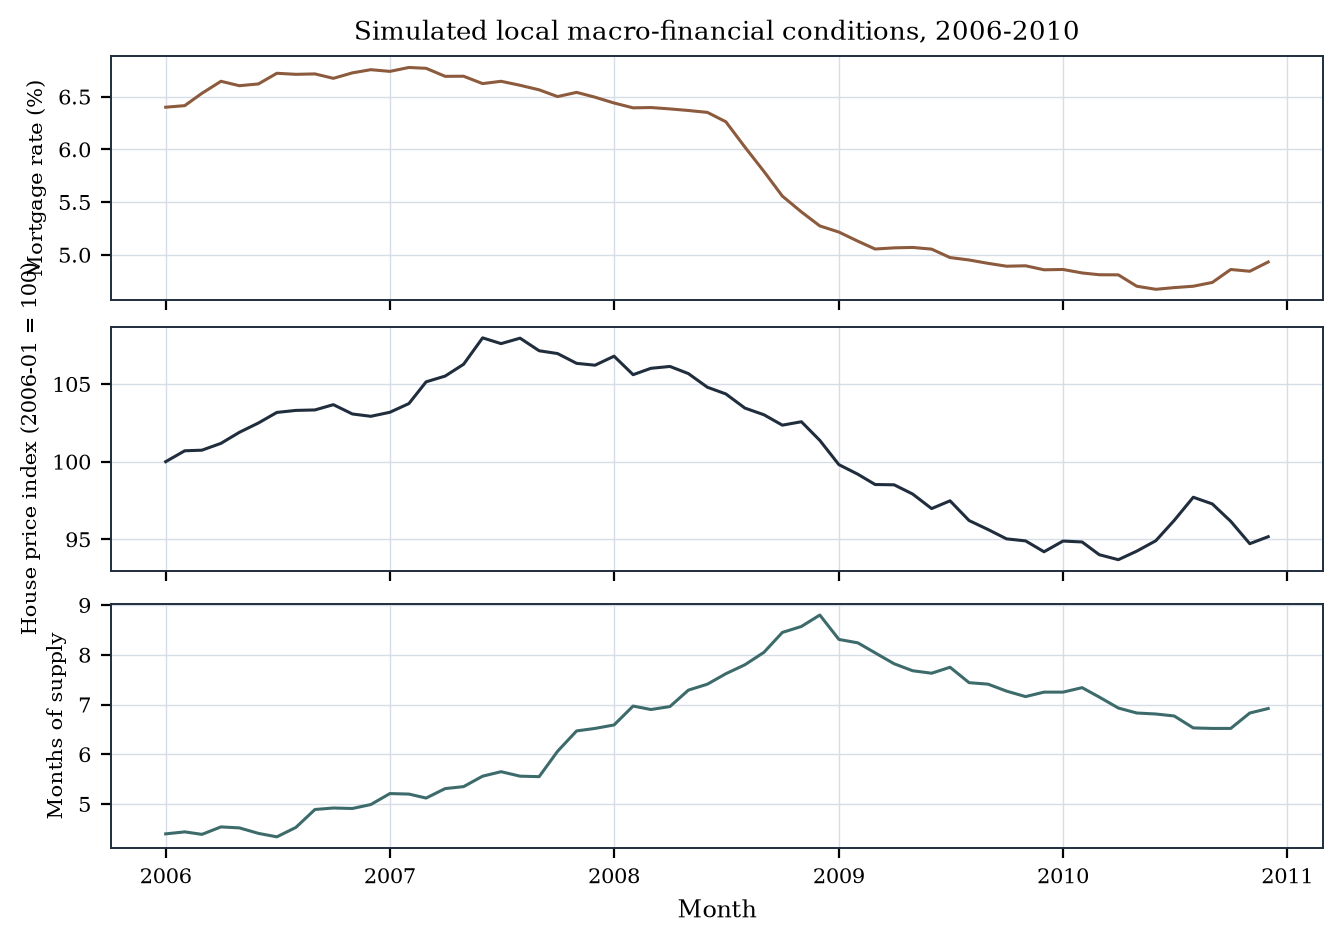
\includegraphics[width=0.74\linewidth]{fig12_macro_trends.png}
\caption{Simulated macro-financial conditions, 2006--2010: the 30-year mortgage rate,
the local house price index (January 2006 = 100) and months of supply. The anchors
reproduce the shape of the United States housing cycle; monthly AR(1) noise prevents
the series from looking mechanically interpolated.}
\label{fig:macro}
\end{figure}

Three pieces of evidence support the realism of the generated context. First,
internal consistency: the amenity score averages 43.5 in tier-1 neighbourhoods, 53.1
in tier 2, 63.0 in tier 3, 73.8 in tier 4 and 85.5 in tier 5, so the measure
separates sub-markets in the direction local knowledge predicts without having been
fitted to prices. Second, external consistency: the generated fields correlate with
price in the expected directions, with crime at $-0.55$, distance to transit at
$-0.37$, distance to school at $-0.28$ and the amenity score at $0.615$ in Pearson
terms and $0.652$ in Spearman terms. Third, behavioural plausibility: marketing
duration has a median of 31 days and a 90th percentile of 69 days, and it lengthens
for weaker locations, lower-quality properties, winter listings and high-interest-rate
periods, which is the pattern platforms actually observe.

The argument has a limit, revisited in Section~\ref{sec:recommendations}. Because
the generator encodes assumptions, the coefficient on a synthetic field measures the
assumption as much as the market. A strong amenity coefficient is evidence that the
model recovered the simulated gradient, not that a one-point improvement raises the
price of a specific house by a specific amount. Causal language is therefore avoided,
and the synthetic fields are treated as controls that improve conditional accuracy
rather than as policy levers.

\subsection{Leakage controls}

Target leakage is the most common way for a housing model to report a flattering and
worthless result. Three controls are enforced. The generator never reads the sale
price; variables recorded after the transaction closes (sale condition, sale type,
days on market, listing date, sale year and month) are excluded from the model even
though they are present in the analytical table; and the neighbourhood tier is not
supplied as an input, so the model must infer sub-market effects from observed
location and amenity fields. The exclusion list is maintained in configuration and
exercised by the test suite, so a change that reintroduces a leaking column fails a
test rather than silently inflating accuracy.

% ---------------------------------------------------------------------------
\section{Exploratory Data Analysis}
\label{sec:eda}
% ---------------------------------------------------------------------------

\subsection{The distribution of sale price}

Figure~\ref{fig:price-dist} shows the target before and after transformation. The
raw distribution is unimodal and strongly right-skewed, with a long tail above
400,000 \USD{} and a skewness of 1.881. The mean (180,933 \USD) sits 17,933 \USD{}
above the median (163,000 \USD), visible in the figure as the separation between the
reference lines. The natural logarithm reduces skewness to 0.122 and kurtosis from
6.52 to 0.80, compressing the influence of extreme observations without discarding
them. The transformation is not a complete cure: a Shapiro--Wilk test on the logged
target rejects normality ($p = 1.2\times10^{-7}$), which matters because a model
assuming Gaussian errors in log space would produce intervals that are too narrow in
the tails. This is one reason the project adopts conformal rather than analytical
intervals.

\begin{figure}[htbp]
\centering
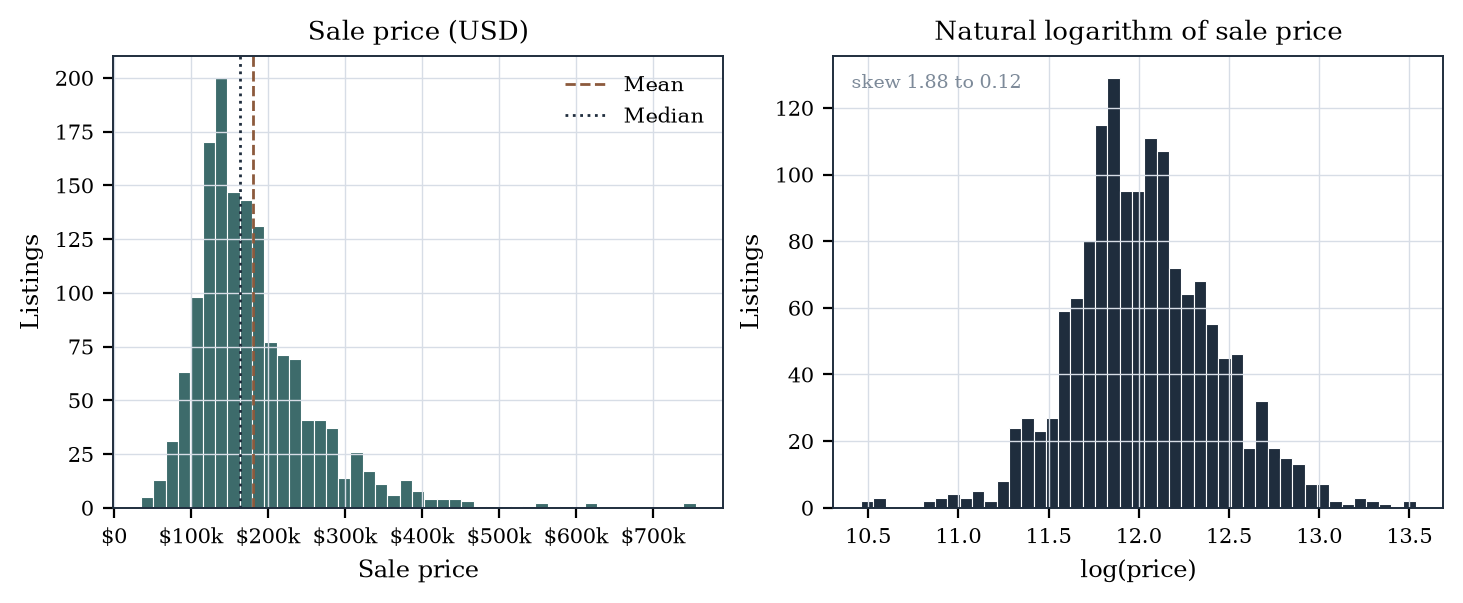
\includegraphics[width=0.90\linewidth]{fig01_price_distribution.png}
\caption{Sale price in \USD{} (left) and its natural logarithm (right). The dashed
and dotted rules mark the mean and median. Logarithmic scaling reduces skewness from
1.881 to 0.122.}
\label{fig:price-dist}
\end{figure}

\subsection{Location and sub-market segmentation}

Location is the strongest organising structure in the data.
Figure~\ref{fig:neigh} orders the 25 neighbourhoods by median price and shows
substantial separation. The median ranges from 88,000 \USD{} in MeadowV and 103,000
\USD{} in IDOTRR to 301,500 \USD{} in NoRidge and 315,000 \USD{} in NridgHt, a ratio
of more than three to one within one small city. The ordering matches local
knowledge: newer northern and western neighbourhoods with larger lots sit at the top,
older eastern and southern neighbourhoods at the bottom.

\begin{figure}[htbp]
\centering
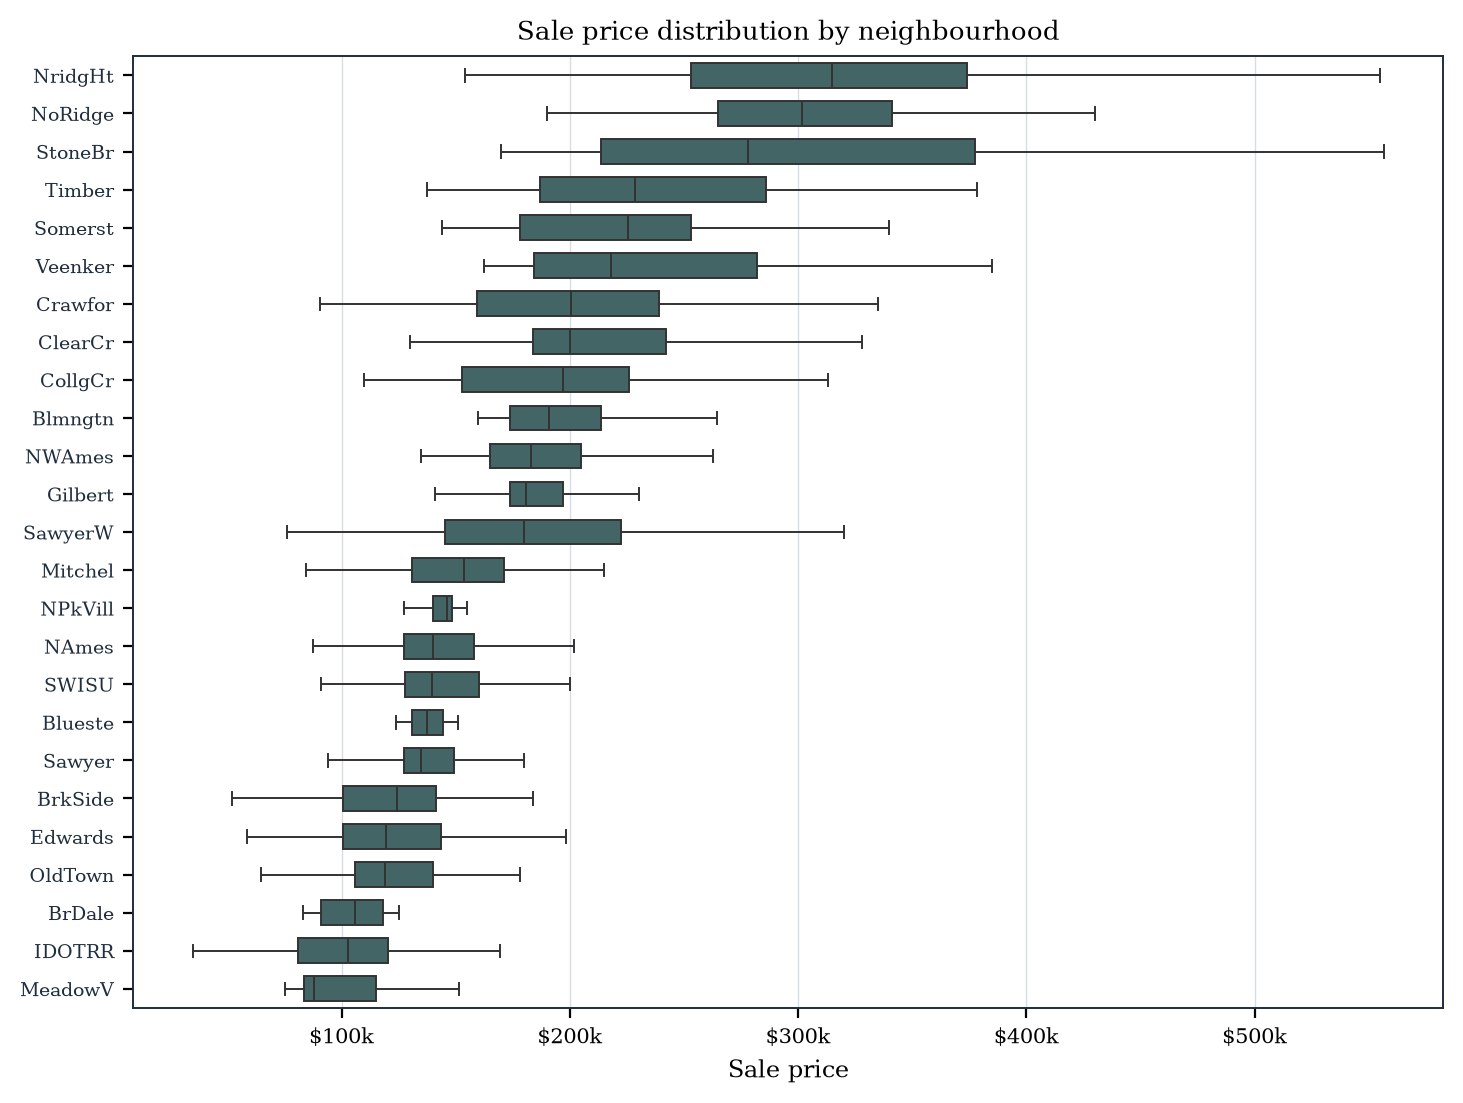
\includegraphics[width=0.60\linewidth]{fig02_price_by_neighbourhood.png}
\caption{Distribution of sale price by neighbourhood, ordered by median. Boxes span
the interquartile range, the central rule marks the median, and whiskers extend to
1.5 times the interquartile range.}
\label{fig:neigh}
\end{figure}

Aggregating the neighbourhoods into five tiers, the prior used by the synthetic
generator, produces a monotone gradient in median price: 109,000 \USD{} for tier 1,
125,500 for tier 2, 148,000 for tier 3, 196,750 for tier 4 and 306,000 for tier 5.
The gradient is not an artefact of the tier construction, because the tier never
enters the model; it is a compact description of how much price variation in this
market is locational. It also implies that a single global error metric will hide
large differences in dollar error across sub-markets, a point developed in
Section~\ref{sec:models}.

\subsection{Property type, architectural style and age}

Property type adds a dimension that location alone does not capture.
Single-family detached homes dominate with 1,218 of 1,458 transactions and a median
of 167,900 \USD. Attached end units (TwnhsE, 114 listings) have a near-identical
median of 172,200 \USD, whereas interior townhouses (43 listings, median 137,500
\USD), duplexes (52 listings, 135,980 \USD) and conversions (2fmCon, 31 listings,
127,500 \USD) trade at a discount of roughly 18 to 24 per cent to detached stock
(Figure~\ref{fig:ptype}). Two-storey homes (443 listings, median 190,000 \USD) and
split levels (65 listings, 164,500 \USD) sit above single-storey homes (726 listings,
154,750 \USD). Style is partly a proxy for size and vintage, so its marginal effect
should not be read as a causal premium for height; the practical consequence is that
the listing profile must include building type and style, because pricing a duplex
with a detached-home template would systematically over-value it.

\begin{figure}[htbp]
\centering
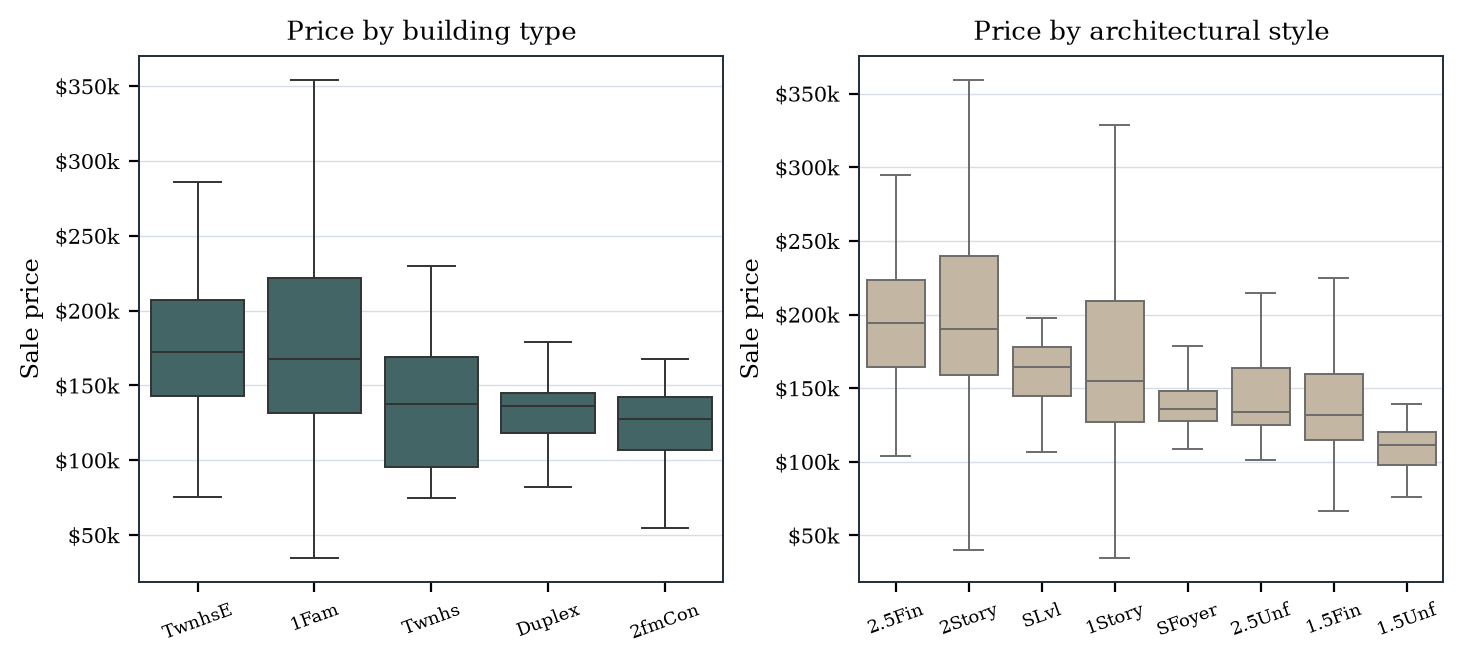
\includegraphics[width=0.88\linewidth]{fig25_price_by_property_type.png}
\caption{Sale price by building type (left) and architectural style (right). Detached
single-family homes and two-storey styles occupy the upper part of the distribution;
interior townhouses, duplexes and conversions occupy the lower part.}
\label{fig:ptype}
\end{figure}

Age is negatively associated with price at the margin: age at sale correlates at
$-0.524$ and years since remodelling at $-0.510$. The relationship is not monotone
across construction cohorts (Table~\ref{tab:decade}). Median prices rise from 108,000
\USD{} for the 1870s cohort to 224,000 \USD{} for the 2000s cohort, but the 1920s
cohort (115,000 \USD) is cheaper than the 1910s cohort (128,750 \USD), and median
floor area rises from around 1,200--1,300 square feet in the mid-twentieth century to
1,636 square feet in the 2000s. Part of the apparent age premium is therefore a size
premium, and the multivariate model is needed to separate the two. Renovation is a
separate signal: the scope indicator correlates negatively with price ($-0.199$)
because deep renovations concentrate in the oldest stock, where a major renovation is
evidence that a house needed one.

\begin{table}[htbp]
\centering
\caption{Sale price and floor area by construction decade, selected cohorts. The 2010
cohort contains a single transaction and is reported for completeness only.}
\label{tab:decade}
\small
\begin{tabular}{@{}lrrr@{}}
\toprule
\textbf{Construction decade} & \textbf{Listings} & \textbf{Median price (\USD)} & \textbf{Median area (sqft)} \\
\midrule
1870s & 2 & 108,000 & 1,689 \\
1910s & 58 & 128,750 & 1,566 \\
1920s & 97 & 115,000 & 1,208 \\
1950s & 167 & 136,000 & 1,196 \\
1970s & 188 & 147,500 & 1,273 \\
1990s & 163 & 204,000 & 1,716 \\
2000s & 385 & 224,000 & 1,636 \\
2010 & 1 & 394,432 & 1,856 \\
\bottomrule
\end{tabular}
\end{table}

\subsection{Price drivers, amenity access and collinearity}

Figure~\ref{fig:corr} ranks the marginal correlations with price. Size and quality
dominate: total floor area (0.833), overall quality (0.796), above-grade living area
(0.735), basement area (0.651) and garage capacity (0.641) are the strongest positive
associates, while the crime index ($-0.551$), age at sale ($-0.524$) and distance to
transit ($-0.365$) are the strongest negative ones. The pattern is economically
sensible: buyers pay for space, condition and access, and discount distance and
disamenity.

\begin{figure}[htbp]
\centering
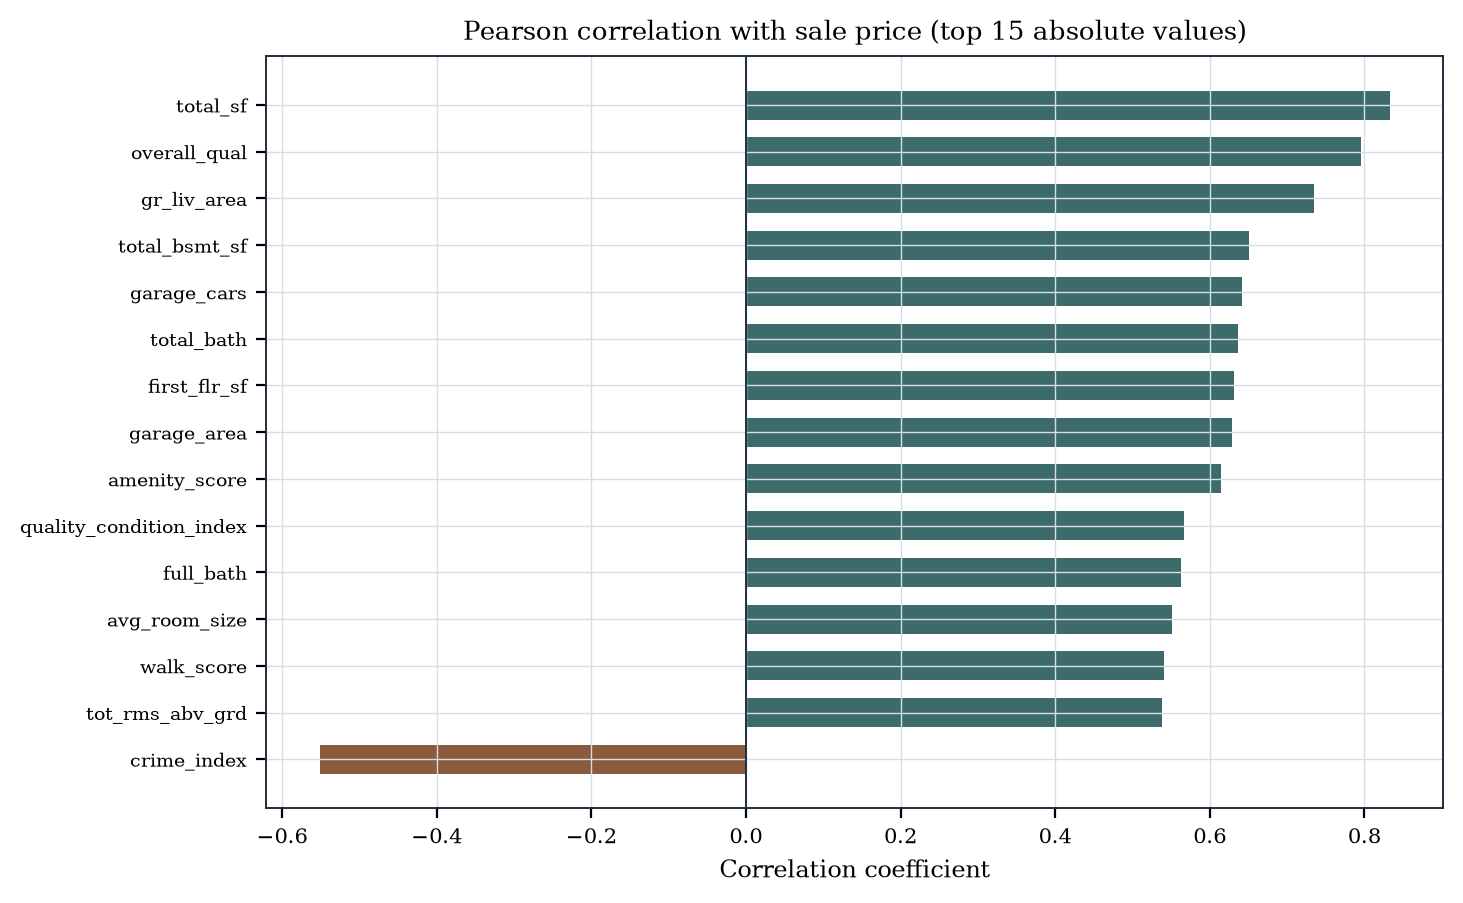
\includegraphics[width=0.88\linewidth]{fig03_price_drivers_correlation.png}
\caption{Pearson correlation of the fifteen attributes most strongly associated with
sale price. Positive associations are dark green, negative associations brown. The
ranking is descriptive and ignores confounding between attributes.}
\label{fig:corr}
\end{figure}

Figure~\ref{fig:amenity} makes the location gradient explicit. Premium neighbourhoods
cluster at high amenity scores and high prices, value neighbourhoods at low scores and
low prices, and the overlap region is where the model earns its keep: properties with
similar amenity access but different structural quality must be separated by the
structural attributes. The figure also exposes heteroscedasticity: the vertical spread
of price at a given amenity score rises from roughly 50,000 \USD{} in the value
segment to more than 300,000 \USD{} in the premium segment. Absolute errors will
therefore be larger for expensive homes even when relative errors are comparable,
which is why the evaluation reports both dollar and percentage errors and why
interval width is expressed as a percentage of the estimate.

\begin{figure}[htbp]
\centering
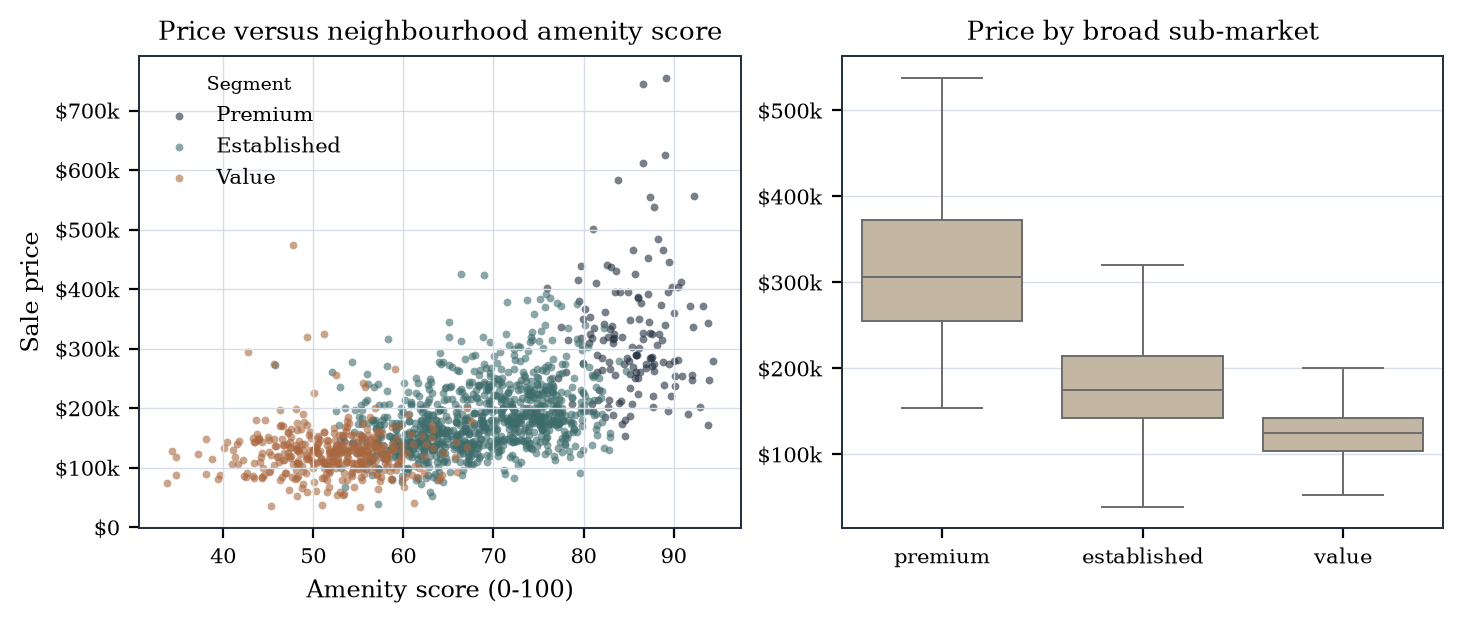
\includegraphics[width=0.88\linewidth]{fig05_amenity_price.png}
\caption{Price against neighbourhood amenity score by sub-market segment (left) and
price within the three segments (right). The association is positive and
heteroscedastic.}
\label{fig:amenity}
\end{figure}

Marginal correlations are a screening device, not a model. Total floor area is a
composite of basement, first-floor and second-floor areas and correlates with
above-grade living area at 0.866; garage area and capacity correlate at 0.887;
construction year and age at sale correlate at $-0.999$ by construction. These
redundancies inflate variance inflation factors and destabilise linear coefficients,
which motivates the pruning described in Section~\ref{sec:features}.

% ---------------------------------------------------------------------------
\section{Data Cleaning}
\label{sec:cleaning}
% ---------------------------------------------------------------------------

The training file contains 7,829 missing cells across nineteen attributes, but the
count alone is misleading. Figure~\ref{fig:missing} shows a characteristic pattern:
the largest gaps belong to features that most houses simply do not have. A pool
quality is missing for 1,453 of 1,460 properties, a miscellaneous feature for 1,406,
an alley for 1,369 and a fence for 1,179. Imputing a mode into these columns would
invent amenities that do not exist; the correct treatment records absence as a level.

\begin{figure}[htbp]
\centering
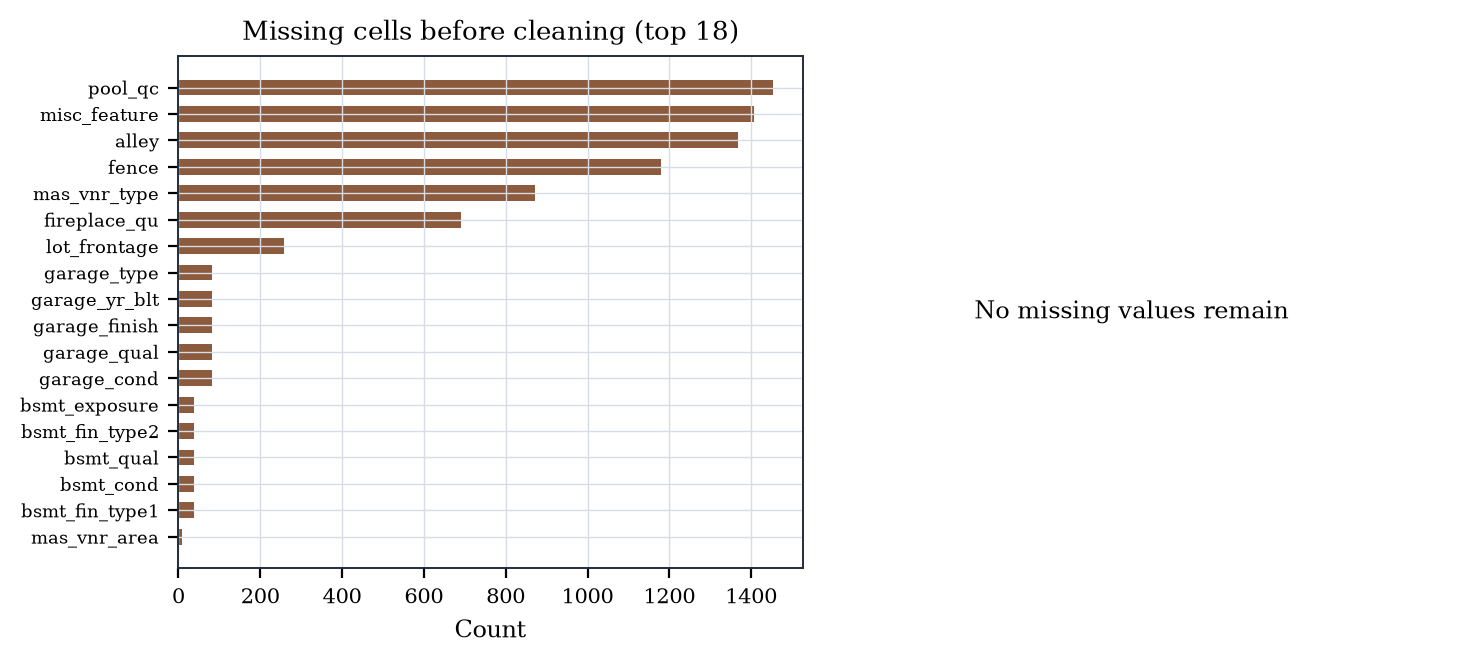
\includegraphics[width=0.86\linewidth]{fig07_missing_values.png}
\caption{Missing cells by attribute before cleaning (eighteen most affected
attributes) and the confirmation that no missing values remain after the rules are
applied.}
\label{fig:missing}
\end{figure}

Three semantics are present, and distinguishing them is the conceptual work of this
module. \emph{Structural absence} means the property does not have the feature, and
the missing value is information: a house without a basement has no basement quality.
\emph{Absent quantity} means the feature exists conceptually but has zero extent: a
house with no garage has zero garage area. \emph{Genuine missingness} means the value
exists but was not recorded, which is the case for lot frontage on 259 properties and
the electrical system on one. Table~\ref{tab:cleaning} records the treatment for each
group.

\begin{table}[htbp]
\centering
\caption{Missing-data treatment by semantic group. Counts refer to the training file.
The total of 7,829 cells is reduced to zero and no row is dropped for missingness.}
\label{tab:cleaning}
\small
\begin{tabularx}{\linewidth}{@{}L{0.22\linewidth}L{0.27\linewidth}rL{0.24\linewidth}@{}}
\toprule
\textbf{Group} & \textbf{Attributes} & \textbf{Cells} & \textbf{Treatment} \\
\midrule
Structural absence & 15 attributes (pool, alley, fence, basement and garage quality, fireplace quality, veneer type) & 7,480 & Literal level ``None'' \\
Absent quantity & Masonry veneer area & 8 & Zero \\
Unstructured categorical & Electrical system & 1 & Training mode \\
Lot frontage & Continuous & 259 & Neighbourhood median, global fallback \\
Garage year & Construction year & 81 & House construction year \\
\midrule
Total & 19 attributes & 7,829 & No missing cells remain \\
\bottomrule
\end{tabularx}
\end{table}

Lot frontage is imputed by neighbourhood rather than globally for a reason. Frontage
is strongly related to neighbourhood type, and the neighbourhood medians range from
21 feet in MeadowV and BrDale to 91 feet in NoRidge. A global median of 69 feet would
assign the same frontage to a dense inner-suburb lot and to a large estate lot, and
would therefore attenuate the relationship between frontage and price.

Outliers are handled by five explicit rules: implausible area--price combinations
(more than 4,000 square feet sold below 300,000 \USD), extreme lot size (above
100,000 square feet), implausible price per square foot (outside 25--500 \USD),
invalid garage year and invalid remodelling year. Only the first removes records: two
transactions, 0.14 per cent of the sample, which are inconsistent with the local
price-per-square-foot distribution and exert disproportionate leverage on a
least-squares fit. The removal applies to training data only; the unlabelled file is
scored in full. The extreme-lot rule flags four observations but removes none,
because a large lot is a genuine market feature rather than a data-entry error, and
the remaining three rules found no violations.

The decision to retain the 61 interquartile-range price outliers (4.2 per cent of the
sample) is equally deliberate. These are expensive houses, not erroneous records, and
deleting them would bias the model against precisely the luxury segment that the
subgroup analysis later identifies as weakest. The log transformation already limits
their influence, and conformal calibration absorbs their effect on interval width.
Removing them would improve the reported average error while making the product worse
for the customers who need it most.

The duplicate check found no exact duplicate records and no duplicated transaction
identifiers, leaving 1,458 rows from the original 1,460. Categorical labels were
canonicalised before validation: whitespace stripped and collapsed, case folded, and
documented spelling variants mapped to a canonical level. No residual inconsistency
survived this pass in the training file, which is reported as zero label variants
fixed. Unknown levels are preserved rather than coerced to the mode, so a genuinely
new category in the unlabelled file does not silently become a frequent one, and the
same mapping is applied at inference time. Every decision in this section is recorded
in \texttt{artifacts/metrics/cleaning\_report.json}, including per-attribute counts,
the neighbourhood medians used for imputation and the rule text for each outlier
check, so the before-and-after comparison can be verified rather than trusted.

% ---------------------------------------------------------------------------
\section{Feature Engineering}
\label{sec:features}
% ---------------------------------------------------------------------------

\subsection{Derived features and the log target}

Eighteen derived variables are computed from the cleaned table. Every one is
row-wise, so the identical transformation applies to a single listing at inference
time and no train--serve skew is possible. Table~\ref{tab:engineered} groups them by
business purpose. The composites exist because several raw attributes measure the
same underlying quantity: usable area is the sum of basement, first-floor and
second-floor area, and bathroom provision is better summarised by a weighted count
that treats a half bathroom as half a full one. Age is expressed as age at sale and
years since remodelling rather than as construction years, because an agent reasons
about how old a house is, not about the calendar year in which it was built.

\begin{table}[htbp]
\centering
\caption{Engineered features by business purpose. The first sixteen are model inputs;
the last two are analysis variables and are excluded from the model matrix.}
\label{tab:engineered}
\small
\begin{tabularx}{\linewidth}{@{}L{0.18\linewidth}L{0.36\linewidth}X@{}}
\toprule
\textbf{Family} & \textbf{Features} & \textbf{Rationale} \\
\midrule
Floor area & \f{total\_sf}, \f{total\_porch\_sf} & Usable covered area; aggregate outdoor amenity space \\
Bathrooms & \f{total\_bath} & Full-bathroom equivalents in one count \\
Age and renovation & \f{age\_at\_sale}, \f{remod\_age}, \f{is\_renovated}, \f{renovation\_scope\_code} & Depreciation and vintage; depth of the last permitted renovation \\
Presence flags & \f{has\_pool}, \f{has\_garage}, \f{has\_fireplace}, \f{has\_second\_floor} & Separates absence of an amenity from a small amount of it \\
Ratios & \f{liv\_area\_ratio}, \f{garage\_area\_ratio}, \f{rooms\_per\_1000sf}, \f{avg\_room\_size} & Development intensity; layout spaciousness \\
Quality & \f{quality\_condition\_index} & Joint effect of quality and maintenance condition \\
Analysis only & \f{price\_per\_sqm}, \f{log\_price} & Reporting metric and target; both use the price and are never inputs \\
\bottomrule
\end{tabularx}
\end{table}

The model is trained on $\log(1 + \text{SalePrice})$. The transformation reduces
skewness from 1.881 to 0.122, it matches the multiplicative structure of housing
prices, and it stabilises the variance of expensive observations so that a 700,000
\USD{} house does not dominate the fit. It also has a consequence that is often
overlooked: because the exponential of a mean log price is not the mean price,
back-transforming with $\exp(\hat{\mu}) - 1$ estimates a conditional median and is
biased low by roughly half the residual variance unless a smearing correction is
applied \citep{hastie2009esl}. No smearing correction is applied here. The
consequence is visible in the diagnostics: the mean signed error is $-853$ \USD, so
the model predicts slightly below the realised price on average. Given that
over-valuation is weighted more heavily in Equation~\eqref{eq:loss}, the direction is
commercially convenient, but the report presents it as a bias rather than as
accuracy.

\subsection{Encoding, selection and collinearity}

Numerical inputs are median-imputed and standardised; categorical inputs are imputed
with the most frequent level and one-hot encoded with a minimum frequency of ten
observations, so rare levels are grouped instead of producing indicators estimated on
a handful of rows. Unseen levels at inference time are ignored rather than treated as
errors. Tree learners use either the same one-hot matrix without scaling or
LightGBM's native categorical handling, so preprocessing is part of the fitted
pipeline and is identical offline and online. After encoding the matrix contains 102
inputs: 40 categorical, 29 structural, 12 structural composites, 10 neighbourhood, 5
macro-financial, 2 locational and 4 age or renovation variables.

Selection proceeds in three steps. Four uninformative columns are removed because
they are constant or almost constant in the sample: street type, utilities, pool
quality and the raw renovation flag, which duplicates the engineered
\f{is\_renovated} flag. A second step applies the leakage policy described below.
The third measures multicollinearity on the 55-feature identifiable numeric core, and
this step repays attention. The deliberate algebraic composites are excluded from the
computation, because including a composite together with its components would make
the design rank-deficient and produce infinite factors that say nothing about the
data. The remaining core is pruned iteratively: the feature with the largest factor
above ten is removed, factors are recomputed, and the process repeats until none
exceeds the threshold. Eight features are removed and 47 are retained, with a maximum
retained factor of 8.95 for garage area as a share of lot area. The eight removed features begin with the amenity score
(351.1), which is almost a linear combination of the distances, ratings and crime
variables from which it was composed, and continue with \f{has\_pool} (62.7),
\f{mortgage\_rate\_pct} (57.3), \f{second\_flr\_sf} (42.6), \f{tot\_rms\_abv\_grd}
(41.5), \f{local\_unemployment\_pct} (40.8), \f{quality\_condition\_index} (39.8)
and \f{renovation\_scope\_code} (13.4).



The pruning is a diagnostic of redundancy, not a filter applied to the model matrix.
Features such as the number of rooms above grade and the quality--condition index
remain inputs, and the regularised linear model handles their collinearity by
shrinking and distributing coefficient mass across correlated variables. The
practical implication is interpretive: individual coefficients on collinear features
must not be read as independent effects, which is why the report relies on grouped
SHAP shares rather than on raw coefficient magnitudes.

The leakage exclusion list is enforced in configuration and asserted by the test
suite. It removes direct functions of the target (\f{SalePrice}, \f{log\_price},
\f{price\_per\_sqm}); variables recorded only after the transaction closes
(\f{sale\_condition}, \f{sale\_type}); marketing outcomes (\f{days\_on\_market},
\f{listing\_date}); sale timing replaced by the macro context (\f{sale\_year},
\f{sale\_month}, \f{yr\_sold}, \f{mo\_sold}); and identifiers. The most consequential
exclusion is days on market. It is plausibly predictive, with a Spearman correlation
of $-0.435$ with price, but it is observed only after a listing has sold and is
therefore unavailable when the estimate is produced.

% ---------------------------------------------------------------------------
\section{Model Development and Evaluation}
\label{sec:models}
% ---------------------------------------------------------------------------

\subsection{Validation design}

All eight families are evaluated on identical folds, features and preprocessing, so
that differences in error are attributable to the estimator. The protocol is
five-fold cross-validation with shuffling and seed 42, producing one out-of-fold
prediction for each of the 1,458 transactions. Preprocessing is fitted inside each
fold as part of the scikit-learn pipeline \citep{pedregosa2011sklearn}, so imputation
and scaling statistics are computed without the validation rows, and the same
pipeline object is later serialised for serving.

Hyperparameters are tuned inside the cross-validation loop. The three regularised
linear models use exhaustive grid search over their penalty paths: eight values of
$\alpha$ for ridge and lasso and eighteen combinations of $\alpha$ and the $L_1$
ratio for the elastic net \citep{tibshirani1996lasso,zou2005elasticnet}. The four
tree ensembles use randomised search, which is more efficient than a grid when only a
few hyperparameters matter \citep{bergstra2012random}: 14 draws for the random
forest, 10 for gradient boosting, 22 for XGBoost and 30 for LightGBM
\citep{chen2016xgboost,ke2017lightgbm}. The selection rule is the lowest out-of-fold
root mean squared error in log space; business metrics are reported alongside but do
not influence selection. Selecting on the same out-of-fold predictions that are then
reported is optimistically biased \citep{varma2006bias}, which is why the temporal
holdout of Section~\ref{sec:models} is treated as the independent check.

\subsection{Benchmark of eight regression families}

Table~\ref{tab:benchmark} presents the results. The regularised linear models occupy
the first four places. The elastic net is selected with an out-of-fold RMSE of 20,019
\USD, a mean absolute error of 13,537 \USD{} and an $R^2$ of 0.9365; lasso is 3.6
\USD{} behind in root mean squared error, a difference far below any meaningful
threshold that should be read as a tie between the two sparse linear specifications.
Ridge and ordinary least squares follow at 20,172 and 21,135 \USD. The boosted
ensembles reach 22,471 \USD{} (XGBoost), 22,518 \USD{} (LightGBM) and 22,689 \USD{}
(gradient boosting), and the random forest is last at 25,725 \USD.

\begin{table}[htbp]
\centering
\caption{Out-of-fold performance of the eight regression families under identical
five-fold cross-validation. The selected model is shown in bold. Dollar figures are
in \USD; the tolerance column is the share of estimates within $\pm$15,000 \USD{} of
the realised price.}
\label{tab:benchmark}
\small
\begin{tabular}{@{}lrrrrrr@{}}
\toprule
\textbf{Model} & \textbf{RMSE} & \textbf{MAE} & \textbf{MAPE} & \textbf{$R^2$} & \textbf{Within} & \textbf{Cost} \\
 & & & (\%) & & \textbf{15k (\%)} & (\USD) \\
\midrule
\textbf{Elastic net} & \textbf{20,019} & \textbf{13,537} & \textbf{7.98} & \textbf{0.9365} & \textbf{69.7} & \textbf{16,708} \\
Lasso & 20,023 & 13,625 & 8.02 & 0.9365 & 69.5 & 16,848 \\
Ridge & 20,172 & 13,753 & 8.13 & 0.9356 & 69.3 & 17,005 \\
Linear regression & 21,135 & 14,500 & 8.56 & 0.9293 & 65.8 & 18,009 \\
XGBoost & 22,471 & 14,419 & 8.25 & 0.9200 & 68.3 & 17,564 \\
LightGBM & 22,518 & 14,665 & 8.49 & 0.9197 & 66.5 & 17,964 \\
Gradient boosting & 22,689 & 14,674 & 8.49 & 0.9185 & 65.9 & 17,925 \\
Random forest & 25,725 & 15,803 & 9.02 & 0.8952 & 66.5 & 18,923 \\
\bottomrule
\end{tabular}
\end{table}

The result is informative rather than surprising. With a log-transformed target and
a feature set whose main effects are strong and largely additive, a well-regularised
linear model has little bias left to remove, while a tree ensemble pays a variance
price for interactions the sample cannot support \citep{hastie2009esl}. The random
forest is worst by a clear margin: averaging many deep trees smooths the prediction
surface and cannot extrapolate beyond the range of the training target, which
penalises exactly the expensive properties the residual analysis identifies as
difficult. The ranking by mean asymmetric cost is not identical to the ranking by
RMSE, because XGBoost over-values less often than linear regression, but the elastic
net still has the lowest cost of the eight.

The selected estimator combines an $L_1$ penalty, which sparsifies, with an $L_2$
penalty, which stabilises correlated features \citep{zou2005elasticnet}. Its largest
standardised coefficients belong to the infrequent-zoning indicator ($-0.268$), rooms
above grade ($0.072$), the infrequent-functional indicator ($-0.071$), the Crawford
neighbourhood ($0.068$), the quality--condition index ($0.057$) and total floor area
($0.056$). A coefficient on a rare indicator applies to few rows and reflects the
composition of that group rather than a general mechanism, which is why the
discussion of drivers relies on SHAP rather than on raw coefficients.

\subsection{Calibrated prediction intervals}

Point estimates alone are insufficient, because the platform must know when to
publish a valuation and when to escalate it. Intervals are produced by split
conformal prediction \citep{angelopoulos2023conformal}: the absolute residuals of the
out-of-fold predictions in log space are collected and the quantile at level
$\lceil (n+1)(1-\alpha)\rceil/n$ is computed, which provides finite-sample marginal
coverage under exchangeability. The quantiles are 0.1173 log points at the 80 per
cent level and 0.1648 at the 90 per cent level, and the interval is obtained by
adding and subtracting the quantile in log space before back-transforming, which
makes it multiplicative and approximately proportional in dollars.

Table~\ref{tab:coverage} reports empirical coverage. Overall coverage is 0.801 and
0.901 at the two nominal levels, as close to exact as a sample of this size allows.
The segment results are less comfortable: the entry band is covered at 0.718 against
a nominal 0.80, a shortfall of 8.2 percentage points, and the luxury band at 0.783;
at the 90 per cent level the entry band reaches 0.833 and the luxury band 0.870. The
mid and upper bands are over-covered. Interval widths are stable at 23.7 per cent of
the estimate for the 80 per cent interval and 33.3 per cent for the 90 per cent
interval.

\begin{table}[htbp]
\centering
\caption{Empirical coverage of the split-conformal intervals, overall and by price
band, computed on the out-of-fold predictions used for calibration. A negative gap
means the interval covers fewer sales than its nominal level.}
\label{tab:coverage}
\small
\begin{tabular}{@{}llrrr@{}}
\toprule
\textbf{Level} & \textbf{Segment} & \textbf{Coverage} & \textbf{Gap} & \textbf{Mean width (\% of price)} \\
\midrule
80\% & All & 0.801 & $+0.001$ & 23.7 \\
80\% & Entry ($<$130k) & 0.718 & $-0.082$ & 24.6 \\
80\% & Mid (130k--200k) & 0.836 & $+0.036$ & 23.5 \\
80\% & Upper (200k--300k) & 0.831 & $+0.031$ & 23.3 \\
80\% & Luxury ($\geq$300k) & 0.783 & $-0.017$ & 22.6 \\
90\% & All & 0.901 & $+0.001$ & 33.3 \\
90\% & Entry ($<$130k) & 0.833 & $-0.067$ & 34.7 \\
90\% & Mid (130k--200k) & 0.941 & $+0.041$ & 33.1 \\
90\% & Upper (200k--300k) & 0.909 & $+0.009$ & 32.8 \\
90\% & Luxury ($\geq$300k) & 0.870 & $-0.030$ & 31.8 \\
\bottomrule
\end{tabular}
\end{table}

\begin{figure}[htbp]
\centering
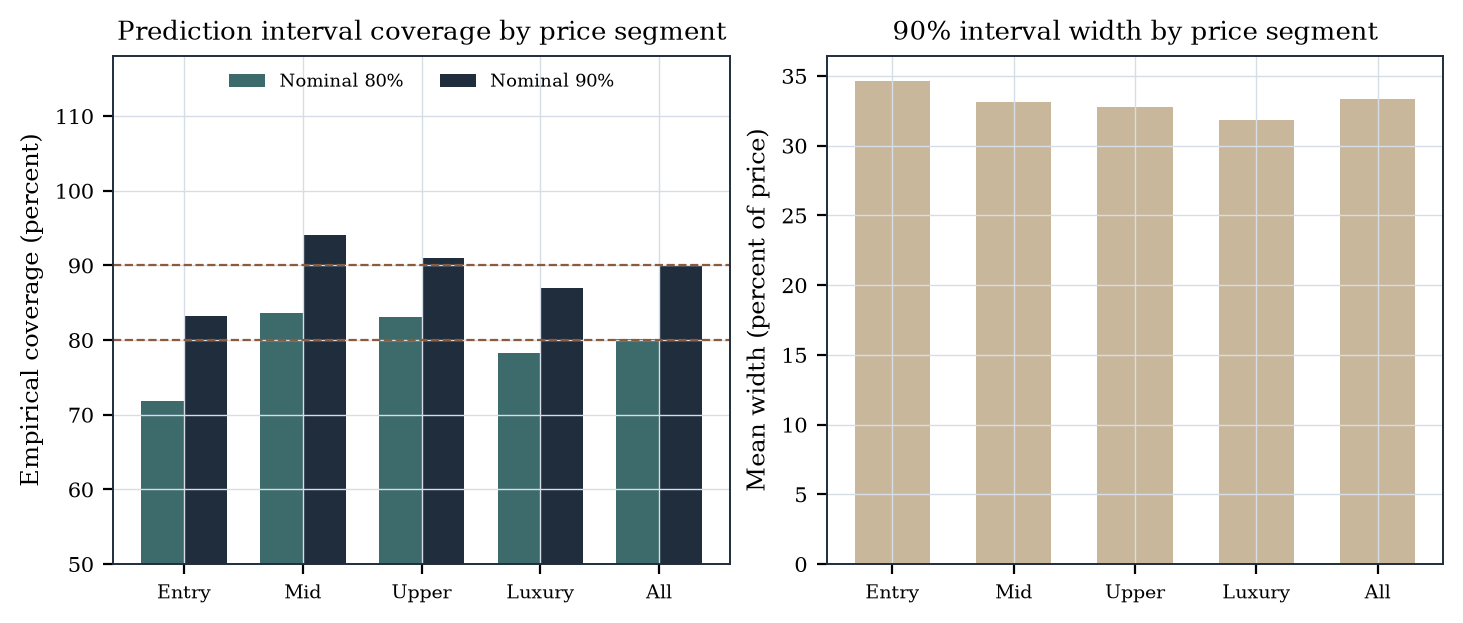
\includegraphics[width=0.88\linewidth]{fig20_interval_coverage.png}
\caption{Empirical coverage of the 80 and 90 per cent conformal intervals by price
band (left) and mean width of the 90 per cent interval as a percentage of price
(right). The entry band under-covers while the mid and upper bands over-cover.}
\label{fig:coverage}
\end{figure}

Figure~\ref{fig:coverage} shows the same pattern graphically. Two caveats accompany
the table. Coverage is measured on the same out-of-fold residuals from which the
quantiles were calibrated, so the overall figures are in-sample for the calibration
step and optimistic as estimates of future coverage; the independent evidence is the
monitoring replay in Section~\ref{sec:monitoring}. And a single global quantile
cannot be correct for both a 90,000 \USD{} starter home and a 500,000 \USD{}
property, because the scale of dollar error differs by a factor of three.
Segment-conditional conformal calibration, or conformalised quantile regression
\citep{romano2019cqr}, would address this and is the highest-value extension of the
uncertainty layer.

\subsection{Residual diagnostics and subgroup performance}

Residual diagnostics are summarised in Figure~\ref{fig:residual}. The mean log residual is $-0.00055$ with a standard
deviation of 0.1112, so the fit is unbiased on average in log space and the typical
multiplicative error is about 11 per cent. The distribution is left-skewed
($-1.141$) and fails the Jarque--Bera test decisively (statistic 2,861, $p<0.001$)
\citep{jarque1980}; the Breusch--Pagan test rejects homoscedasticity (LM statistic
131.9, $p<0.001$) \citep{breusch1979}. Error is also concentrated: the worst five per
cent of cases account for 22.1 per cent of total absolute error, the 90th percentile
of absolute error is 29,122 \USD{} and the maximum is 138,115 \USD. The mean absolute
error of 13,537 \USD{} therefore conceals a tail that matters for escalation
decisions.



\begin{figure}[htbp]
\centering
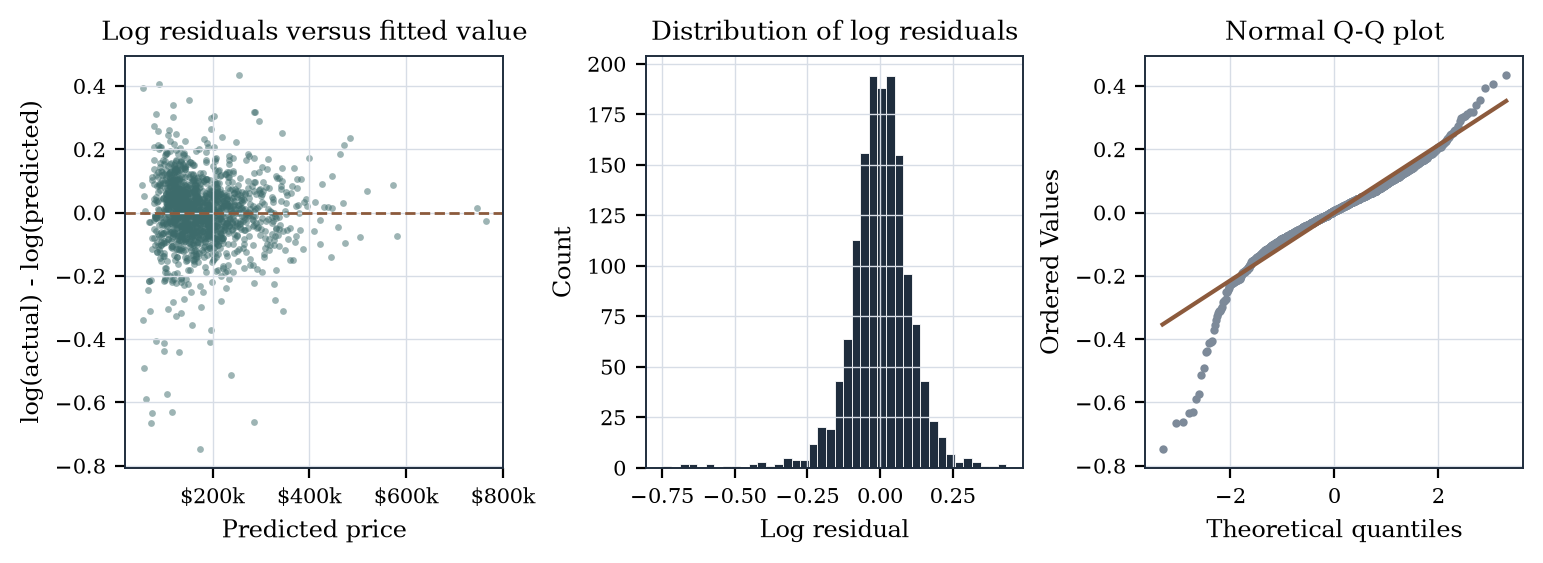
\includegraphics[width=\linewidth]{fig17_residual_diagnostics.png}
\caption{Residual diagnostics: log residuals against fitted value (left),
distribution of log residuals (centre) and normal quantile--quantile plot (right).
The left tail is longer than the right and the quantile plot departs from the
reference line at both ends.}
\label{fig:residual}
\end{figure}

The diagnostics carry three implications. The left skew means the model occasionally
over-predicts substantially, the expensive direction under Equation~\eqref{eq:loss}.
Heteroscedasticity invalidates analytical Gaussian intervals, which justifies the
conformal approach. And the concentration of error means that a product reporting only
the mean would understate the tail risk that drives review decisions.

Table~\ref{tab:subgroup} disaggregates error by neighbourhood segment and price band.
Dollar error rises steeply with price: mean absolute error is 11,581 \USD{} in value
neighbourhoods, 12,892 \USD{} in established neighbourhoods and 23,035 \USD{} in
premium neighbourhoods, and it rises from 10,295 \USD{} in the entry band to 31,238
\USD{} in the luxury band. Relative bias tells the opposite story and is the more
actionable signal. The entry band is over-predicted by 4.70 per cent, so the platform
would systematically quote first-time buyers a price above what they eventually pay,
while the luxury band is under-predicted by 3.92 per cent, transferring value away
from sellers of expensive homes.

\begin{table}[htbp]
\centering
\caption{Subgroup performance of the selected model. Neighbourhood segments group
tiers 1--2 as value, tier 3 as established and tiers 4--5 as premium. Bias is the
mean signed error as a percentage of the sale price; a positive value indicates
over-prediction.}
\label{tab:subgroup}
\small
\begin{tabular}{@{}lrrrr@{}}
\toprule
\textbf{Segment} & \textbf{Sales} & \textbf{RMSE (\USD)} & \textbf{MAE (\USD)} & \textbf{Bias (\%)} \\
\midrule
Value neighbourhoods & 389 & --- & 11,581 & $+1.34$ \\
Established neighbourhoods & 926 & --- & 12,892 & $+0.54$ \\
Premium neighbourhoods & 143 & --- & 23,035 & $+0.08$ \\
\midrule
Entry band ($<$130k) & 365 & 14,521 & 10,295 & $+4.70$ \\
Mid band (130k--200k) & 658 & 15,413 & 10,973 & $+0.08$ \\
Upper band (200k--300k) & 320 & 21,864 & 16,147 & $-0.91$ \\
Luxury band ($\geq$300k) & 115 & 41,499 & 31,238 & $-3.92$ \\
\bottomrule
\end{tabular}
\end{table}

The asymmetry between dollar error and relative bias is the central evaluation
insight of this project. Judged by mean absolute error the model is much worse for
expensive homes; judged by percentage bias it is systematically cheap for expensive
homes and systematically generous for inexpensive ones. Both facts are true and have
different remedies. The first is a scale effect that no model can eliminate entirely,
because expensive properties are heterogeneous and thinly traded. The second is a
calibration defect that segment-specific review thresholds or an asymmetric objective
can address.

\subsection{Drivers of the valuation}

Figure~\ref{fig:shap} ranks the global drivers by mean absolute SHAP value, computed
with the linear explainer for the elastic net and aggregated from one-hot columns
back to their parent attributes \citep{lundberg2017shap}. Rooms above grade
contributes 8.73 per cent of total explanation mass, total floor area 6.51, the
quality--condition index 6.31, average room size 4.51, age at sale 3.41, basement
finish type 3.19, neighbourhood latitude 3.05 and total bathrooms 2.76. Aggregated by
family, structural attributes account for 43.35 per cent, categorical attributes for
27.82, structural composites for 15.87, age and renovation for 6.21, location for
3.20, neighbourhood amenities for 2.40 and macro-financial context for 1.14.

\begin{figure}[htbp]
\centering
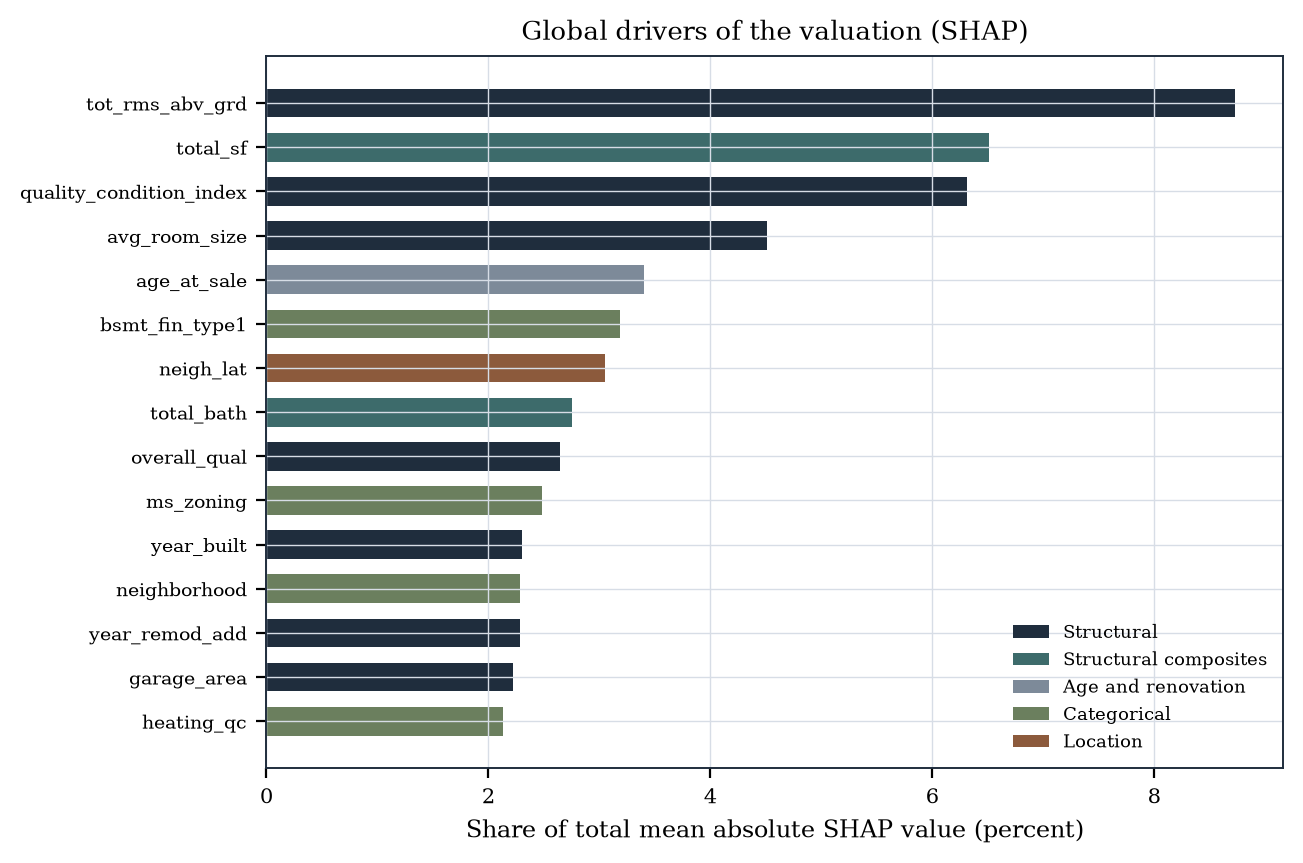
\includegraphics[width=0.74\linewidth]{fig18_global_drivers.png}
\caption{Global drivers of the valuation by mean absolute SHAP value as a share of
the total, coloured by feature family. Structural and categorical attributes
dominate; simulated contextual fields carry a smaller but non-trivial share.}
\label{fig:shap}
\end{figure}

The decomposition supports the business narrative that quality, space and condition
drive value, and it also disciplines it. Location enters indirectly through
neighbourhood indicators and latitude rather than through a single interpretable
premium, and the macro block contributes only 1.14 per cent of in-sample attribution.
That should not be read as evidence that macro conditions do not matter: SHAP values
describe how the fitted model uses each feature across the training distribution,
which contains modest and correlated macro variation. The monitoring
study shows that when the macro block moves outside that distribution, prediction
levels shift and coverage collapses. In-sample attribution and out-of-sample
sensitivity are different questions, and the report keeps them separate.

\subsection{Temporal holdout}

Cross-validation measures interpolation within the sample, not behaviour on future
listings. A temporal holdout provides a stricter test: the model is refitted on the
1,283 sales completed in 2006--2009 and evaluated on the 175 sales completed in 2010,
which are never used for tuning or selection. Root mean squared error rises to 22,269
\USD{} and mean absolute error to 14,820 \USD, with an $R^2$ of 0.9229 and a MAPE of
8.71 per cent. The tolerance hit rate falls to 63.4 per cent and the over-valuation
rate to 36.0 per cent, so the holdout model is both slightly less accurate and
markedly more conservative than the cross-validated one. The 11 per cent degradation
in root mean squared error is the honest estimate of the cost of forecasting forward
in this market, and it remains inside the targets of Table~\ref{tab:kpis}. Part of
the degradation is compositional rather than temporal, because 2010 sales are
concentrated in the first half of the year and the sample is small. The report quotes
the out-of-fold result, the holdout and the monitoring replay rather than the most
flattering of the three.

% ---------------------------------------------------------------------------
\section{Deployment}
\label{sec:deployment}
% ---------------------------------------------------------------------------

\subsection{Architecture and API contract}

The system has three runtime components (Table~\ref{tab:components}). The inference
service is a FastAPI application that loads the serialised pipeline at start-up and
exposes point estimates, intervals, batch scoring, local explanations and the latest
monitoring summary. The valuation console is a Streamlit application \citep{streamlit2026} that renders
a listing form for agents and a read-only monitoring view. Monitoring artefacts are
generated offline by a scheduled script and served both as a static HTML dashboard
and through the API, so the console never computes statistics itself.

\begin{table}[htbp]
\centering
\caption{Runtime components of the deployed valuation product. Paths are relative to
the repository root.}
\label{tab:components}
\small
\begin{tabularx}{\linewidth}{@{}L{0.16\linewidth}L{0.32\linewidth}L{0.07\linewidth}X@{}}
\toprule
\textbf{Component} & \textbf{Entry point} & \textbf{Port} & \textbf{Purpose} \\
\midrule
Valuation API & \path{src/revaluation/api/main.py} & 8000 & Estimates, intervals, batch scoring, explanations, monitoring summary \\
Valuation console & \path{app/streamlit_app.py} & 8501 & Agent-facing form, performance and monitoring views \\
Monitoring artefacts & \path{scripts/06_run_monitoring.py} & --- & Drift report, alerts, static HTML dashboard \\
\bottomrule
\end{tabularx}
\end{table}

Two design decisions matter. The API is stateless apart from the model artefact, so
it scales horizontally without session affinity. The console calls the API through
the \texttt{VALUATION\_API\_URL} variable but falls back to an in-process copy of the
same pipeline when the API is unreachable, which keeps a single-service deployment
demonstrable on free tiers where a sleeping API would make the console appear broken;
both paths use the identical pipeline object, so the fallback cannot diverge in
preprocessing.

Table~\ref{tab:endpoints} lists the interface. Validation is declarative through
Pydantic models, and only four fields are required: neighbourhood, overall quality,
above-grade living area and year built. Every other field has a documented default,
so an agent can obtain an estimate from an incomplete listing rather than being
blocked by a long form, and the response records which assumptions were applied.

\begin{table}[htbp]
\centering
\caption{HTTP interface of the valuation API. Interactive OpenAPI documentation is
served at \texttt{/docs} by the framework \citep{fastapi2026}.}
\label{tab:endpoints}
\small
\begin{tabularx}{\linewidth}{@{}L{0.09\linewidth}L{0.25\linewidth}X@{}}
\toprule
\textbf{Method} & \textbf{Path} & \textbf{Purpose} \\
\midrule
GET & \texttt{/health} & Liveness plus model-loaded flag \\
GET & \texttt{/model/info} & Model card, version and validation metrics \\
POST & \texttt{/predict} & Point estimate, 80 and 90 per cent intervals, confidence class \\
POST & \texttt{/predict/batch} & Up to 200 listing profiles per request \\
POST & \texttt{/explain} & Local SHAP contributions for one profile \\
GET & \texttt{/monitoring/summary} & Latest drift, performance and alert summary \\
\bottomrule
\end{tabularx}
\end{table}

The prediction response contains the estimate, both intervals, a confidence class, a
confidence score, the relative 90 per cent interval width, the model name and version,
the assumptions applied and a timestamp. The class is derived from the relative
half-width of the 90 per cent interval: at most 0.18 is high confidence, at most 0.30
is moderate, and anything wider is low and routed to a valuer, which implements the
escalation policy of Section~\ref{sec:business}. An exact request and response are
reproduced in Appendix~\ref{app:api}.

\subsection{The valuation console and packaging}

Figure~\ref{fig:console} shows the console after a request. Inputs are grouped into
location and transaction date, structure and condition, and an optional
neighbourhood-amenity section, so an agent who knows only the basics can still obtain
a valuation. The result panel reports the point estimate, both intervals and the
confidence assessment, and the lower panel lists the local contributions that moved
this particular estimate. For the illustrated profile, a 1975 house in CollgCr with
quality 6, condition 5, 1,500 square feet of living area and a 2005 remodelling, the
response is 146,412 \USD{} with an 80 per cent interval of 130,213--164,626 \USD, a
90 per cent interval of 124,164--172,646 \USD{} and a high confidence classification
with a score of 0.67.

\begin{figure}[htbp]
\centering
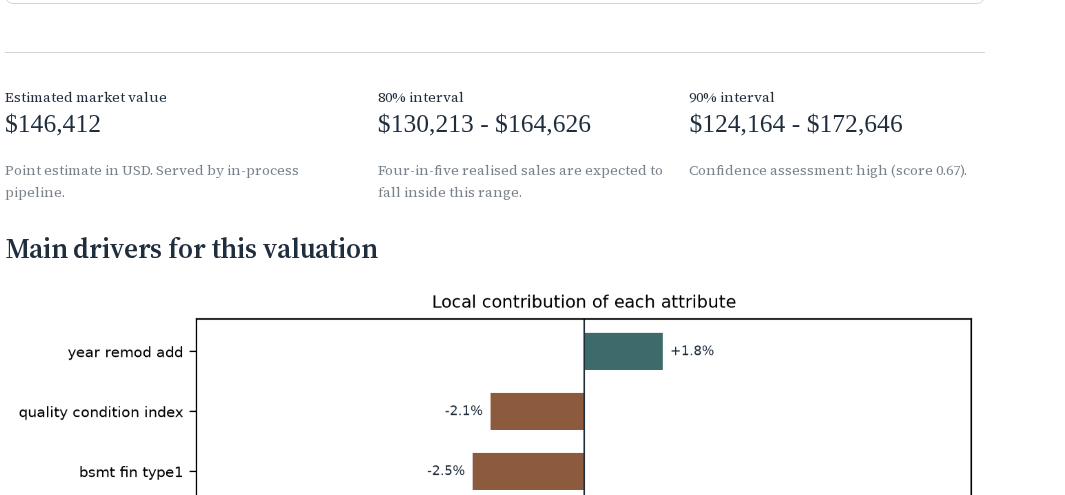
\includegraphics[width=0.95\linewidth]{ui_result_panel.png}
\caption{Result panel of the Streamlit valuation console after a request, cropped
from the full-window capture to keep the output legible. The panel reports the point
estimate with both conformal intervals, the confidence assessment and the local
attribution of the leading drivers.}
\label{fig:console}
\end{figure}

The console also provides a model-performance page and a monitoring page that read
the archived metrics and alerts, so a non-technical stakeholder can inspect the
evidence behind the numbers without opening a notebook. This matters for adoption:
the valuation is useful only if an agent can see how often it has been right.

Two container images are provided: the API image serves the application on the port
given by \texttt{PORT} (default 8000), and the console image does the same for
Streamlit on 8501. Neither trains a model at start-up, so cold starts are dominated
by process startup. A Compose file starts both services, a Render blueprint declares
the two web services with build commands and health checks, and a Hugging Face
Spaces variant uses the Docker SDK on port 7860. Both free tiers impose
sleep-on-inactivity behaviour and a 512 MB ceiling, which the system fits.

\subsection{Verification status and the public-URL question}

The complete system has been verified locally. The health endpoint returns a healthy
status with the model loaded, the information endpoint returns the model card, the
prediction endpoint returns the response in Appendix~\ref{app:api}, the batch and
explanation endpoints return well-formed payloads, and the monitoring endpoint
returns the latest summary once the monitoring script has run. The console renders
the form, calls the service, displays the intervals and the local attribution, and
the static monitoring dashboard is generated without error.

No public URL is claimed. The Render blueprint and the Hugging Face configuration are
complete and the procedure is documented, but provisioning either service requires
the account credentials of the repository owner, which were not available in the
development environment. The team chose not to publish a link that could not be kept
alive, and this report does not present a local address as if it were public. The
remaining work is administrative: authenticate to the hosting account, connect the
repository, set \texttt{VALUATION\_API\_URL} on the console service and confirm the
health check. Until that is done, the deployment criterion of the brief is satisfied
in substance but not in form, and the report states this plainly rather than implying
otherwise.

% ---------------------------------------------------------------------------
\section{Post-Deployment Monitoring}
\label{sec:monitoring}
% ---------------------------------------------------------------------------

\subsection{A temporal replay}

The competition's unlabelled file carries no prices, so it cannot support performance
monitoring: drift can be measured, but realised error cannot. The project therefore
builds a genuine replay. The reference model is the selected estimator refitted on the
945 sales completed before January 2009, the vintage that would have been in
production then; its out-of-fold root mean squared error is 20,888 \USD{} and its
MAPE 7.88 per cent. The stream is the 513 sales completed between January 2009 and
July 2010, split into four equal-volume windows of 128 or 129 transactions. Realised prices are treated as
labels that arrive only after a window closes, mirroring the delay between listing
activity and recorded deeds. The design has the property that matters: the monitoring
period is strictly outside the reference model's training data, so accuracy and
coverage measured on the stream are honest out-of-sample quantities. It also has a
limitation that must be stated: the stream is a replayed history, so the monitoring
layer is exercised against a realistic sequence of sales but not against the
operational failures, such as late or duplicated data, that a production feed would
present.

\subsection{What is monitored}

Four families of signal are tracked. Input drift is measured for numeric features by
the population stability index (PSI) on ten reference quantiles, with the
Kolmogorov--Smirnov statistic as a distribution-free cross-check; categorical drift
uses PSI on level proportions with total variation distance; prediction drift is the
PSI of the score distribution, which captures the shift users would notice; and
realised performance is measured by rolling RMSE, MAE, MAPE, mean signed bias, the
business tolerance rate and the empirical coverage of both intervals. PSI is
interpreted with the conventional bands: below 0.10 stable, 0.10 to 0.20 moderate and
0.20 or above significant \citep{siddiqi2006,yurdakul2018psi}. Because the index sums
weighted divergences over bins, empty bins are floored at $10^{-4}$ and the outer
edges are widened to infinity, which prevents a single unseen value from producing an
unbounded index.

\subsection{Window-level results}

Table~\ref{tab:monitoring-windows} reports the observed replay. Accuracy degrades
modestly: root mean squared error rises from 22,306 \USD{} in the first two windows to
23,395 \USD{} in the third and 21,839 \USD{} in the fourth, which corresponds to RMSE
ratios of 1.068, 1.068, 1.120 and 1.046 against the reference. No window crosses the
1.2 ratio that would trigger the accuracy rule, and mean absolute percentage error
stays between 9.14 and 9.63 per cent.

\begin{table}[htbp]
\centering
\caption{Observed replay of the 2009--2010 stream through four equal-volume
chronological windows. The reference model was fitted on 945 sales from January 2006
to December 2008 (out-of-fold RMSE 20,888 \USD).}
\label{tab:monitoring-windows}
\small
\begin{tabular}{@{}lrrrrrr@{}}
\toprule
\textbf{Window} & \textbf{Sales} & \textbf{RMSE} & \textbf{MAE} & \textbf{MAPE} & \textbf{Bias} & \textbf{90\%} \\
 & & (\USD) & (\USD) & (\%) & (\%) & \textbf{coverage} \\
\midrule
W1, 2009-01 to 2009-06 & 129 & 22,306 & 14,813 & 9.41 & $-0.16$ & 0.891 \\
W2, 2009-06 to 2009-09 & 128 & 22,306 & 16,143 & 9.14 & $-1.57$ & 0.875 \\
W3, 2009-09 to 2010-04 & 128 & 23,395 & 15,977 & 9.63 & $-2.52$ & 0.836 \\
W4, 2010-04 to 2010-07 & 128 & 21,839 & 16,048 & 9.34 & $-4.99$ & 0.797 \\
\bottomrule
\end{tabular}
\end{table}

Calibration behaves very differently from accuracy. The 90 per cent interval covers
89.1 per cent of sales in the first window, 87.5 in the second, 83.6 in the third and
79.7 in the fourth; the 80 per cent interval falls from 76.7 to 65.6 per cent over the
same sequence. The intervals are not becoming wider or narrower in any material way;
the distribution of realised prices is moving away from the calibrated residuals.
This is the failure mode that a point-estimate dashboard would miss entirely, and it
is the strongest argument for monitoring calibration alongside accuracy.

\subsection{Drift}

Figure~\ref{fig:drift} shows the PSI by window for twelve informative features and
for the prediction distribution, alongside the window-level performance in
Table~\ref{tab:monitoring-windows}.
Between five and seven of the 43 monitored features exceed the 0.20 threshold in every
window, and the same block is responsible each time: mortgage rate, house price index,
its year-on-year change, local unemployment and months of supply. This is precisely
the block simulated to follow the 2006--2011 cycle, and the reference vintage ends in
December 2008, so the stream contains the steepest part of the rate decline and the
bottom of the price index. The model has no comparable observations in its training
window, which is why both the PSI and the coverage respond.

\begin{figure}[htbp]
\centering
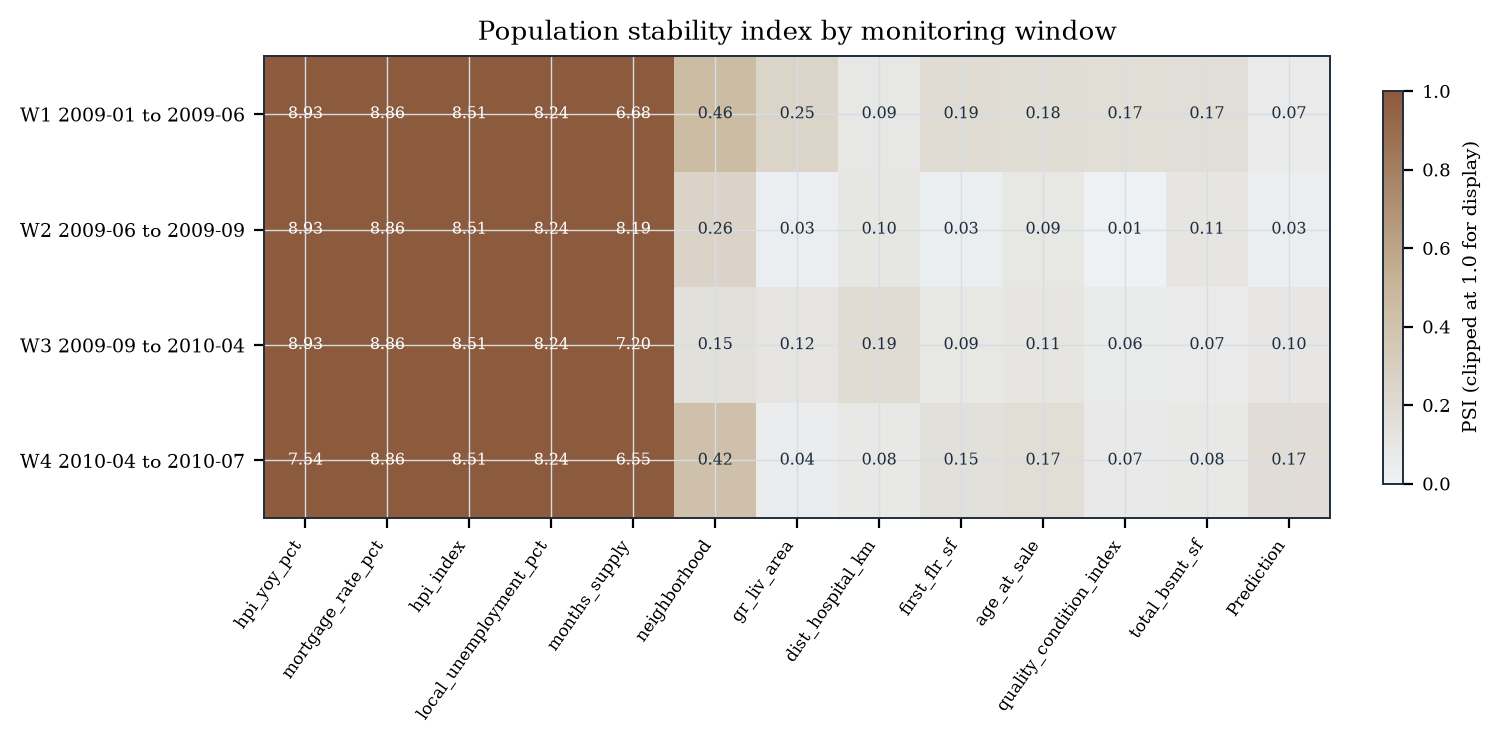
\includegraphics[width=\linewidth]{fig22_drift_heatmap.png}
\caption{Population stability index by monitoring window for the most informative
features and for the prediction distribution. Values are clipped at 1.0 for display;
the untruncated macro values reach 8.9 because the reference window contains almost
none of the later rate and index levels.}
\label{fig:drift}
\end{figure}

Two details deserve interpretation. The neighbourhood indicator also drifts, with a
PSI of 0.46 in the first window and 0.42 in the fourth, because the mix of
neighbourhoods sold changes between periods: a moderate compositional change that a
platform would investigate before concluding that the market itself had moved.
Second, prediction drift rises from 0.066 to 0.174, moderate rather than significant,
even though input drift on the macro block is extreme, because that block carries only
1.14 per cent of in-sample attribution. Prediction drift alone would have understated
the problem; it is the combination of drift, coverage and bias that identifies the
failure.


\subsection{Alert rules and the retraining decision}

Nine rules are evaluated on every run, grouped into input drift, prediction drift,
accuracy, coverage and bias, with sustained versions of the accuracy, coverage and
bias rules elevated to critical severity (Table~\ref{tab:rules}). The observed replay
raises four R1 warnings, two R4 coverage warnings and one critical R7 alert for
sustained coverage erosion. R5 does not fire, because the final-window bias of $-4.99$
per cent sits just inside the 5 per cent threshold, and the accuracy rules do not
fire because no window exceeds 1.2 times the reference RMSE.

\begin{table}[htbp]
\centering
\caption{Monitoring and retraining policy. A critical alert opens a retraining
ticket. The observed replay triggers R1, R4 and R7; the stress scenario additionally
triggers R5.}
\label{tab:rules}
\small
\begin{tabularx}{\linewidth}{@{}L{0.05\linewidth}L{0.31\linewidth}L{0.10\linewidth}X@{}}
\toprule
\textbf{Rule} & \textbf{Condition} & \textbf{Severity} & \textbf{Action} \\
\midrule
R1 & At least 3 features with PSI $\geq$ 0.20 & Warning & Review input pipeline and market context \\
R2 & Prediction PSI $\geq$ 0.20 & Warning & Confirm shift is explained by market moves \\
R3 & Window RMSE $>$ 1.2 $\times$ reference & Critical & Inspect worst errors, prepare retraining \\
R4 & 90\% coverage $<$ 0.85 & Warning & Recalibrate conformal quantiles \\
R5 & $|$mean signed bias$|$ $>$ 5\% & Warning & Verify the macro feed and sale dates \\
R6 & R3 in two consecutive windows & Critical & Retrain \\
R7 & R4 in two consecutive windows & Critical & Recalibrate and retrain if erosion persists \\
R8 & R5 in two consecutive windows & Critical & Retrain with recent data \\
R9 & R1 in two consecutive windows & Warning & Schedule retraining for the next release \\
\bottomrule
\end{tabularx}
\end{table}

The decision is to retrain now. The first action is to recalibrate the conformal
quantiles on recent residuals, because the point estimates remain within tolerance
while the uncertainty layer no longer covers its nominal level; the second is to refit
on the most recent 24 months of labelled data, promoting the new model only if both
out-of-fold RMSE and coverage improve. Recalibration precedes retraining because the
two failures are different.

\subsection{Stress scenario, tooling and reproducibility}

To verify that the alerting machinery reacts to a sharper shift, the reference model
is scored on a counterfactual stream in which the mortgage rate rises by 1.5
percentage points, inventory rises by one month of supply and amenity distributions
improve by 60 per cent, while recorded prices are held at their observed values. The
scenario is a controlled perturbation, not a forecast. Under stress, ten to twelve
features drift in the first two windows rather than five to seven, the RMSE ratio
peaks at 1.152, 90 per cent coverage falls to 81.2 per cent and bias reaches $-5.23$
per cent, firing R5 in addition to R7. The accuracy ratio still does not cross 1.2,
so even a severe context shift would be invisible to a purely accuracy-based
monitor.

The announcement recommends the Evidently library for the dashboard
\citep{evidently2026}. The team evaluated it and found that the released version
depends on internal pandas interfaces removed in pandas 3.1; adopting it would have
required pinning the project to an older pandas release and diverging from the
dependency set used by training and serving. The component was therefore implemented
directly with the statistical primitives Evidently uses (PSI, Kolmogorov--Smirnov,
chi-square) and rendered as a static HTML dashboard plus a Streamlit view. The
trade-off is explicit: less out-of-the-box functionality, but consistent dependencies
and thresholds that can be audited line by line against Table~\ref{tab:rules}. The replay is deterministic, so re-running the script
reproduces every number in Table~\ref{tab:monitoring-windows} and every alert in
\texttt{artifacts/monitoring/alerts.json}. Version-pinned artefacts, scheduled
execution and archived reports are the practices that make post-deployment behaviour
auditable \citep{sculley2015,gama2014conceptdrift}.

% ---------------------------------------------------------------------------
\section{Pricing Strategy, Limitations and Future Work}
\label{sec:recommendations}
% ---------------------------------------------------------------------------

\subsection{From model output to pricing policy}

The model should be used as a pricing anchor with an explicit range, not as a single
authoritative number. The 80 per cent interval is the natural object to show an
agent: at the median listing it spans roughly a quarter of the estimate, wide enough
to contain a normal negotiation but narrow enough to be informative. The point
estimate should be presented as the centre of that range, and the 90 per cent interval
should drive the escalation decision, because it is the interval whose coverage the
monitoring layer tracks.

The subgroup results imply that a single review threshold is the wrong policy. The
entry band is over-predicted by 4.70 per cent, so a first-time buyer is likely to see
a price above what the property eventually achieves; a conservative adjustment of the
published anchor in that band, or automatic review of entry-band estimates, would
reduce the reputational cost of systematic generosity. The luxury band is
under-predicted by 3.92 per cent with a mean absolute error of 31,238 \USD, more than
three times the entry-band error, so luxury estimates should be routed to a valuer by
default regardless of their nominal confidence. The premium neighbourhood segment
shows almost no bias ($+0.08$ per cent) but a mean absolute error of 23,035 \USD: it
is unbiased on average and unreliable in individual cases, which is exactly the
situation in which a wide interval rather than a point estimate should drive the
conversation.

The confidence classes already implement part of this policy. An estimate whose 90
per cent half-width is at most 18 per cent of the point estimate is high confidence
and may be published directly; between 18 and 30 per cent it is moderate and should
be reviewed for high-value listings; above 30 per cent it is low and must be
reviewed. The segment rules should be layered on top of the class rather than
replacing it, because the two capture different risks: the class captures uncertainty
about the individual property, the segment captures known bias in part of the market.

Two further recommendations follow. The interval width is itself a commercial signal:
a wide interval indicates a heterogeneous micro-market or an unusual property, and it
can be shown to the agent as a prompt to request an appraisal rather than as a defect.
And the model should not be used to advise on renovation: renovation accounts for
6.21 per cent of explanation mass, but the synthetic variables are constructed from
the assessor's remodelling year and the coefficients reflect that construction, so a
claim that a kitchen refurbishment adds a specific percentage to value is not
supported. Finally, the economics should be stated in business units: at the observed
mean asymmetric cost of 16,708 \USD{} per listing, every 1,000 valuations carry
roughly 16.7 million \USD{} of weighted pricing error. That is a historical average
rather than a forecast of savings, but it makes clear that a one-point improvement in
the tolerance hit rate is worth more than a small reduction in mean absolute error.

\subsection{Limitations}

The most important limitation is the sample. With 1,458 transactions and 25
neighbourhoods, the model cannot estimate fine interactions, and the luxury band rests
on 115 sales. Comparing eight families mitigates the risk of a poorly suited
specification, but it cannot create information the sample does not contain.

The second is the synthetic context. The amenity, renovation, marketing and macro
variables encode documented assumptions, and their coefficients measure those
assumptions as much as the Ames market. The realism checks in Section~\ref{sec:data}
show that the generated fields behave plausibly, but plausibility is not validation
against an external source. A production system would replace them with licensed
amenity data, county deed records and a live macro feed, and the model would have to be
re-estimated on those inputs.

The third concerns the error distribution. Log residuals are left-skewed and
heteroscedastic, and the worst five per cent of cases account for 22.1 per cent of
total absolute error, so a single global conformal quantile cannot be correct across
the price range; the entry band under-covers by 8.2 percentage points.

The fourth is temporal. The sample covers a single housing cycle and the model has
never observed a high-interest-rate regime. The replay shows that when the macro
context moves outside the reference window, coverage collapses even though accuracy
holds; after a structural break the model would need recalibration before it could be
trusted, and the retraining policy is the mechanism for doing so.

Two methodological caveats belong here as well. The reported out-of-fold metrics are
computed on the same predictions used to select the model, so they are optimistically
biased by a small amount; the temporal holdout is the independent check and shows an
11 per cent degradation in root mean squared error. The conformal coverage figures
are likewise measured on the calibration residuals, with the monitoring replay as the
independent evidence. Neither caveat undermines the conclusions, but both separate an
honest evaluation from a flattering one.

\subsection{Future work}

Table~\ref{tab:future} lists the extensions the team considers most valuable, in
priority order. The first two address defects in the released system; the remainder
extend its scope. The ranking is by expected business value per unit of effort, not by
methodological novelty.

\begin{table}[htbp]
\centering
\caption{Prioritised future work, with the defect or opportunity it addresses and the
expected benefit.}
\label{tab:future}
\small
\begin{tabularx}{\linewidth}{@{}L{0.042\linewidth}L{0.30\linewidth}L{0.26\linewidth}X@{}}
\toprule
\textbf{No.} & \textbf{Extension} & \textbf{Addresses} & \textbf{Expected benefit} \\
\midrule
1 & Segment-conditional conformal calibration or conformalised quantile regression & Entry and luxury under-coverage & Correct coverage within price bands, not only on average \\
2 & Train on the asymmetric loss (expectile regression or weighted objective) & Loss is reported but not optimised & Align the estimate with the 1.5:1 business cost \\
3 & Public deployment with authentication, rate limiting and health checks & No live URL; open CORS in the demonstration build & Satisfies the deployment criterion; protects the service \\
4 & Replace synthetic context with licensed amenity, deed and macro feeds & Coefficients reflect simulated assumptions & External validity and defensible driver analysis \\
5 & Spatial comparable-sales features and sub-neighbourhood location & Location is represented only by indicators and centroid latitude & Sharper pricing in heterogeneous neighbourhoods \\
6 & Automated retraining with shadow evaluation and promotion gates & Manual retraining decision & Faster recovery after drift, with controlled risk \\
7 & Data-quality monitoring for late, duplicated or malformed listings & The replay assumes a clean feed & Detects operational failures before they reach the model \\
\bottomrule
\end{tabularx}
\end{table}

The first item is the most consequential. The current intervals are honest on average
and wrong in the tails, and the entry band is where the product is most likely to be
used by people least able to absorb a pricing error. Mondrian conformal prediction,
which calibrates within each price band, or conformalised quantile regression, which
adapts interval width to the local error scale, would fix the defect with modest
implementation effort and no change to the point estimator
\citep{romano2019cqr,angelopoulos2023conformal}. The second item is conceptually simple
but requires care: optimising the asymmetric loss directly will push predictions
downward, and the resulting model must be evaluated on coverage and tolerance as well
as on weighted cost, or it will simply learn to under-quote.

% ---------------------------------------------------------------------------
\section{Conclusion}
\label{sec:conclusion}
% ---------------------------------------------------------------------------

This project set out to answer a practical question for a listing platform: what is a
property worth at the moment it is listed, and how much confidence should anyone place
in that number? The answer delivered here is an elastic net on the logarithm of sale
price, trained on 1,458 cleaned Ames transactions and 21 documented synthetic
contextual fields, wrapped in split-conformal intervals, exposed through an API and a
Streamlit console, and monitored by a replay of the 2009--2010 market. The model
explains 93.7 per cent of out-of-fold price variance, prices a typical property within
13,537 \USD{} of its realised value, and meets every accuracy, tolerance and
calibration target set at the start of the project.

Three conclusions are more useful than the headline metrics. First, on a small and
well-measured tabular sample, a regularised linear model can beat gradient-boosted
trees, and the benchmark shows the margin clearly. Second, accuracy and calibration
are separate properties that can fail independently: the replay shows a model that
stays within its accuracy tolerance while its 90 per cent interval covers only 79.7
per cent of sales by the final window, and the retraining policy fires on the coverage
rule rather than on the accuracy rule. Third, aggregate metrics conceal commercially
important heterogeneity: the entry band is over-predicted by 4.7 per cent and the
luxury band under-predicted by 3.9 per cent, and a single review threshold would treat
both incorrectly.

The system is verified locally and complete in its configuration, but it is not
publicly deployed, because the cloud account credentials needed to provision a URL
were unavailable to the team. That gap is stated once, here and in
Section~\ref{sec:deployment}, and it is the only deliverable that is not closed. The
analytical work behind the model, the evidence in the artefacts and the monitoring
policy are complete, reproducible from the repository, and ready to be operated by
whoever holds the account.


\clearpage
\appendix
% ---------------------------------------------------------------------------
\section{Data Dictionary Summary}
\label{app:dictionary}
% ---------------------------------------------------------------------------

Every synthetic field is documented with its data type, unit, valid range,
generation logic and the business assumption behind it. The complete dictionary,
including the 81 base columns and the 18 engineered features, is distributed as
\texttt{docs/data\_dictionary.md} and \texttt{docs/data\_dictionary.xlsx} and is
regenerated by the pipeline, so code and documentation cannot drift apart.
Table~\ref{tab:dictionary} reproduces the synthetic fields in abbreviated form as a
reading aid; the dictionary remains the authoritative source. Generation uses seed 42
and is deterministic for a given input order, and the tier variable referred to below
is the documented prior about sub-market desirability, never a model input.

\begin{table}[htbp]
\centering
\caption{Synthetic contextual fields: unit, valid range and abbreviated generation
logic. Ranges are the clipped support of the generated values; the dictionary records
the exact distribution parameters.}
\label{tab:dictionary}
\scriptsize
\begin{tabularx}{\linewidth}{@{}L{0.30\linewidth}L{0.135\linewidth}X@{}}
\toprule
\textbf{Field} & \textbf{Unit and range} & \textbf{Generation logic} \\
\midrule
\f{neigh\_lat} & degrees, 41.99--42.07 & Neighbourhood centroid plus $N(0, 0.0015)$ jitter \\
\f{neigh\_lon} & degrees, $-93.67$ to $-93.60$ & Neighbourhood centroid plus $N(0, 0.0015)$ jitter \\
\f{dist\_school\_km} & km, 0.10--8.00 & Log-normal, median $\exp(1.90 - 0.22t)$, $\sigma=0.35$ \\
\f{dist\_hospital\_km} & km, 0.30--20.00 & Log-normal, median $\exp(5.00 - 0.55t)$, $\sigma=0.30$ \\
\f{dist\_transit\_km} & km, 0.20--15.00 & Log-normal, median $\exp(3.20 - 0.42t)$, $\sigma=0.33$ \\
\f{dist\_park\_km} & km, 0.10--10.00 & Log-normal, median $\exp(1.60 - 0.15t)$, $\sigma=0.30$ \\
\f{school\_rating} & score 1--10 & $\text{clip}(\text{round}(3.2 + 1.15t + N(0,0.9)))$ \\
\f{walk\_score} & score 0--100 & $\text{clip}(\text{round}(18 + 10.5t + N(0,8)))$ \\
\f{crime\_index} & index 0--100 & $\text{clip}(\text{round}(78 - 10.5t + N(0,7)))$ \\
\f{amenity\_density\_1\_5km} & count 0--40 & Poisson with mean $2 + 1.6t$ \\
\f{park\_area\_ha} & hectares 0.05--60 & Log-normal, median $\exp(2.0 + 0.8t)$, $\sigma=0.6$ \\
\f{amenity\_score} & index 0--100 & Weighted composite of distances, ratings and inverse crime, rescaled \\
\f{renovation\_flag} & flag 0--1 & 1 when the remodelling year exceeds the construction year \\
\f{renovation\_scope} & label, None--Major & Major if lag $\geq$ 20 years, moderate if $\geq$ 8, minor otherwise \\
\f{days\_on\_market} & days, 1--365 & Log-normal with tier, quality, month, rate and supply effects; clipped \\
\f{listing\_date} & date, 2005-01--2011-12 & Sale date (day 15) minus days on market \\
\f{mortgage\_rate\_pct} & per cent, 4.30--7.10 & Anchored monthly path (6.40 in 2006-01 to 4.90 in 2010-12) plus AR(1) noise \\
\f{hpi\_index} & index, 94--109 & Anchored monthly path, January 2006 = 100, plus AR(1) noise \\
\f{hpi\_yoy\_pct} & per cent, $-12$ to 12 & Year-over-year change of the price index \\
\f{months\_supply} & months, 3.8--9.5 & Anchored monthly path plus AR(1) noise \\
\f{local\_unemployment\_pct} & per cent, 3.7--6.3 & Anchored monthly path plus AR(1) noise \\
\bottomrule
\end{tabularx}
\end{table}

Two conventions are worth repeating because they are frequently misread. First, the
neighbourhood tier is an input to the generator but never to the model; it encodes an
expert prior about sub-market desirability and is not estimated from sale prices.
Second, a missing value in the base data usually means that a feature is absent rather
than unknown, and the cleaning stage encodes that distinction explicitly
(Section~\ref{sec:cleaning}). Both conventions are enforced in code and described in
the dictionary, so a reader who wants to audit the generation logic has a single
authoritative source.

% ---------------------------------------------------------------------------
\section{Reproducibility and Artefact Map}
\label{app:reproducibility}
% ---------------------------------------------------------------------------

The pipeline is deterministic. Every stage reads the previous stage's artefact and
writes a new one under \texttt{artifacts/}; no stage depends on notebook state or a
manual edit. The commands below are executed from the repository root, and the Python
environment is managed by \texttt{uv} so that the lock file, rather than a
hand-maintained list, defines the dependencies.

\begin{verbatim}
uv sync                                    # create the pinned environment
make pipeline                              # data, cleaning, features, models,
                                           # evaluation, monitoring, dictionary
uv run pytest -q                           # unit and integration tests
uv run ruff check src app scripts tests    # static checks
cd report && latexmk -pdf -interaction=nonstopmode -halt-on-error main.tex

# individual stages, when only one artefact needs regenerating
uv run python scripts/01_generate_context.py
uv run python scripts/02_clean_data.py
uv run python scripts/03_build_features.py
uv run python scripts/04_train_models.py
uv run python scripts/05_run_evaluation.py
uv run python scripts/06_run_monitoring.py
uv run python scripts/07_export_data_dictionary.py

# services (the console falls back to an in-process pipeline if the API is down)
uv run uvicorn revaluation.api.main:app --host 127.0.0.1 --port 8000
uv run streamlit run app/streamlit_app.py
\end{verbatim}

Table~\ref{tab:artefacts} maps the claims in this report to the artefact supporting
them. A reader who wants to check a number can open the corresponding file; a reader
who wants to re-derive it can re-run the stage that produces it.

\begin{table}[htbp]
\centering
\caption{Artefact map: the evidence behind each part of the report. Paths are
relative to the repository root.}
\label{tab:artefacts}
\small
\begin{tabularx}{\linewidth}{@{}L{0.46\linewidth}>{\raggedright\arraybackslash}X@{}}
\toprule
\textbf{Artefact} & \textbf{Content used in this report} \\
\midrule
\path{artifacts/metrics/model_comparison.csv} & Out-of-fold benchmark of the eight families (Table~\ref{tab:benchmark}) \\
\path{artifacts/metrics/training_summary.json} & Selected model, metrics, conformal quantiles, temporal holdout \\
\path{artifacts/metrics/evaluation_diagnostics.json} & Residual tests, SHAP drivers, subgroup performance \\
\path{artifacts/metrics/interval_coverage.csv} & Coverage and width by level and price band \\
\path{artifacts/metrics/cleaning_report.json} & Missing counts, imputation state, outlier rules \\
\path{artifacts/metrics/eda_summary.json} & Distributions, correlations, tiers, decades, VIF summary \\
\path{artifacts/metrics/shap_importance.csv} & Global attribution by raw feature and family \\
\path{artifacts/monitoring/monitoring_summary.json} & Reference vintage, window performance, drift, alerts \\
\path{artifacts/monitoring/alerts.json} & Triggered rules and the retraining decision \\
\path{artifacts/monitoring/monitoring_report.html} & Static monitoring dashboard \\
\path{docs/data_dictionary.md} & Field-level data dictionary (Appendix~\ref{app:dictionary}) \\
\path{artifacts/reports/ui_result.png} & Console screenshot (Figure~\ref{fig:console}) \\
\bottomrule
\end{tabularx}
\end{table}

Two practical notes complete the record. The base competition files are read from
their original directory and never modified, so the pipeline can be re-run against a
fresh download and will produce identical results. The generator and the model both
use a fixed seed of 42; changing it changes the simulated context but not the
structure of the analysis, and the monitoring thresholds and alert rules are
independent of it.

% ---------------------------------------------------------------------------
\section{API Request and Response Example}
\label{app:api}
% ---------------------------------------------------------------------------

The request below was executed against the locally running API. The profile is
deliberately partial: the required fields are the neighbourhood, the overall quality,
the above-grade living area and the year built, and the optional fields supplied are
the remodelling year, overall condition, lot area, basement area, first-floor area,
bathrooms, bedrooms, rooms above grade and the garage.

{\footnotesize
\begin{verbatim}
curl -s -X POST http://127.0.0.1:8000/predict \
  -H "Content-Type: application/json" \
  -d '{"neighborhood": "CollgCr", "overall_qual": 6,
       "gr_liv_area": 1500, "year_built": 1975,
       "year_remod_add": 2005, "overall_cond": 5, "lot_area": 9000,
       "total_bsmt_sf": 800, "first_flr_sf": 900, "full_bath": 2,
       "half_bath": 0, "bedroom_abv_gr": 3, "tot_rms_abv_grd": 7,
       "garage_cars": 2, "garage_area": 480, "fireplaces": 0}'
\end{verbatim}
}

The response contains the point estimate, both conformal intervals, the confidence
classification and the assumptions applied to the omitted fields:

{\footnotesize
\begin{verbatim}
{
  "estimate": 146412.03,
  "currency": "USD",
  "interval_80": [130213.1, 164626.14],
  "interval_90": [124164.33, 172646.02],
  "confidence": "high",
  "confidence_score": 0.6742,
  "relative_interval_width_90": 0.3311,
  "model": "Elastic net",
  "model_version": "2026-11-19T13:20:58+00:00",
  "assumptions": {
    "sale_year": 2010,
    "sale_month": 6,
    "neighbourhood": "CollgCr",
    "derived_context_fields": ["amenity_density_1_5km",
      "amenity_score", "crime_index", "dist_hospital_km",
      "dist_park_km", "dist_school_km", "dist_transit_km",
      "neigh_lat", "neigh_lon", "park_area_ha",
      "school_rating", "walk_score"]
  },
  "generated_at": "2026-11-19T13:50:47+00:00"
}
\end{verbatim}
}

The arithmetic of the confidence class connects the statistical output to the
escalation policy. The 90 per cent interval half-width is
$(172{,}646.02 - 146{,}412.03)/146{,}412.03 = 0.179$, just inside the 0.18 threshold
for high confidence, and the score of 0.6742 follows the service's rule
$1 - 0.179/0.55$. The full relative width of 0.3311 is the quantity stored for
reporting and compared with the segment-level review thresholds recommended in
Section~\ref{sec:recommendations}.

{\footnotesize
\begin{verbatim}
[
  {"feature": "total_sf", "contribution_log": -0.0366,
   "direction": "decreases", "relative_effect_pct": 3.73},
  {"feature": "tot_rms_abv_grd", "contribution_log": -0.0351,
   "direction": "decreases", "relative_effect_pct": 3.57},
  {"feature": "bsmt_fin_type1", "contribution_log": -0.0252,
   "direction": "decreases", "relative_effect_pct": 2.55},
  {"feature": "quality_condition_index", "contribution_log": -0.0212,
   "direction": "decreases", "relative_effect_pct": 2.14}
]
\end{verbatim}
}

The explanation endpoint returns these local contributions for the same profile. All
four are negative because the property is modest relative to the comparison sample:
1,500 square feet of above-grade living area, a basement that the service defaults to
an unfinished finish type, and a quality--condition index of 30 place it below the
centre of its neighbourhood and vintage. The sign and magnitude are consistent with
the global drivers in Figure~\ref{fig:shap}, which is what makes a local explanation
useful to an agent: the attributes that drive the model globally also explain the
individual valuation, so the estimate can be discussed in the language of the listing
rather than the language of the model.


\clearpage
\addcontentsline{toc}{section}{References}
\begingroup
\small
\setlength{\bibsep}{2.6pt}
\bibliographystyle{plainnat}
\bibliography{references}
\endgroup

\end{document}
